
% !TeX root = RJwrapper.tex
\title{The \pkg{segmetric} Package: Metrics for Assessing Segmentation Accuracy for Geospatial Data}
\author{Rolf Simoes, Alber Sanchez, Michelle C. A. Picoli and Patrick Meyfroidt}

\maketitle

\abstract{
Segmentation methods are a valuable tool for exploring spatial data by identifying objects based on images' features. 
However, proper segmentation assessment is critical for obtaining high-quality results and running well-tuned segmentation algorithms Usually, various metrics are used to inform different types of errors that dominate the results. 
We describe a new R package, \CRANpkg{segmetric}, for assessing and analyzing the geospatial segmentation of satellite images. 
This package unifies code and knowledge spread across different software implementations and research papers to provide a variety of supervised segmentation metrics available in the literature. 
It also allows users to create their own metrics to evaluate the accuracy of segmented objects based on reference polygons. 
We hope this package helps to fulfill some of the needs of the R community that works with Earth Observation data. 
}

\section{Introduction}

Earth Observation aims to collect data regarding the Earth's systems at several spatio-temporal resolutions. 
These data allow scientists to understand Earth's processes, such as greenhouse gas emissions and land cover change. 
Segmentation is among the most used unsupervised processing methods for extracting information from satellite imagery~\citep{Hossain2019}. 
Segmentation is the process by which objects are extracted using image features.
This process consists of delineating groups of adjacent pixels with similar characteristics such as intensity, color, and texture. 
Numerous segmentation algorithms are available in the Remote Sensing scientific literature~\citep[see e.g.][]{Kotaridis2021}. 

Assessing segmentation results is difficult due to under and over-segmetation errors.
Undersegmentation occurs when the segmentation algorithm fails to separate a contiguous pixel group while oversegmentation is the opposite, that is, the segmentation algorithm unnecessarily splits a pixel group~\citep{Costa2018}. 
Both under and over-segmentation come with assessment metrics that target segments' characteristics such as area, shape, and position.
One way to assess these errors is to use supervised quality metrics~\citep{Costa2018}.
Supervised metrics compare segments to reference data, measuring their similarity or discrepancy in terms of under and over-segmentation~\citep{Clinton2010}. 

One significant challenge in the domain of Earth Observation data is the scarcity of software tools specifically designed for segmentation assessment. 
While several packages such as \CRANpkg{imageseg} \citep{Niedballa2022}, \CRANpkg{ExpImage} \citep{Azevedo2022}, \CRANpkg{SuperpixelImageSegmentation} \citep{Mouselimis2022}, \CRANpkg{OpenImageR} \citep{Mouselimis2022b}, and \CRANpkg{image.Otsu} \citep{Wijffels2020} enable users to segment images but, when provided, they offer a limited set of facilities to assess the accuracy of the segmentation and some of them are not tailored to the needs of Earth Observation data or applications. 
This often requires users to adapt the code from these packages for their own purposes,
which can be time-consuming and unrelated to their primary research goals.

In this paper, we introduce the \CRANpkg{segmetric} package, which addresses the lack of R tools for assessing segmentation of Earth Observation data and provides a coherent set of metrics that can be used to compare and contrast different assessment methods for evaluating segmentation. Additionally, \CRANpkg{segmetric} provides innovative visualization tools to assist qualitative spatial analysis as well as metrics that can be used to tune and assess segmentation algorithms.

\section{Supervised segmentation metrics}

Supervised metrics use reference data to assess segmentation accuracy. 
These metrics are grouped into two categories: geometric, which use the geometry of the objects (i.e. polygons) to determine the similarity between the segments and the reference data; and thematic, which use instead objects' attributes such as the land cover label associated with each object
~\citep{Costa2018}. The \CRANpkg{segmetric} package focuses on geometric methods that require two sets of polygons as inputs, one for the segments and other for the reference data.

The segments' polygons, denoted by $Y = \{y_j: j = 1, ..., m\}$, are obtained from a segmentation method and the reference polygons, denoted by $X = \{x_i: i = 1, ..., n\}$, are typically collected \textit{in-situ} by specialists. The quality metrics are defined considering different subsets of $X$ and $Y$. The subsets of $Y$ used to compute metrics for each reference $i$ are defined as follows~\footnote{We are following the notation used by~\citet{Clinton2010} and~\citet{Costa2018}}:

\begin{itemize}
 
    \item $\tilde{Y}_{i} \subset{} Y$, where $\tilde{Y}_{i} = \{y_{j}: \rm{area}(x_{i} \cap y_{j}) \neq 0\}$

    \item $Y'_{i} \subset{} Y$, where $Y'_{i} = \{y_{j}: max(\rm{area}(x_{i} \cap y_{j}))\}$

    \item $Y\!a_{i} \subset{} \tilde{Y}_{i}$, where $Y\!a_{i} = \{y_{j}: \rm{centroid}(x_{i}) \:\rm{in}\: y_{j}\}$

    \item $Y\!b_{i} \subset{} \tilde{Y}_{i}$, where $Y\!b_{i} = \{y_{j}: \rm{centroid}(y_{j}) \:\rm{in}\: x_{i}\}$

    \item $Y\!c_{i} \subset{} \tilde{Y}_{i}$, where $Y\!c_{i} = \{y_{j}: \rm{area}(x_{i} \cap y_{j}) / \rm{area}(y_{j}) > 0.5\}$

    \item $Y\!d_{i} \subset{} \tilde{Y}_{i}$, where $Y\!d_{i} = \{y_{j}: \rm{area}(x_{i} \cap y_{j}) / \rm{area}(x_{i}) > 0.5\}$

    \item ${Y}^{*}_{i}$, where ${Y}^{*}_{i} = Y\!a_{i} \cup Y\!b_{i} \cup Y\!c_{i} \cup Y\!c_{i}$

    \item $Y\!cd_{i}$, where $Y\!cd_{i} = Y\!c_{i} \cup Y\!d_{i}$

    \item $Y\!e_{i} \subset{} \tilde{Y}_{i}$, where $Y\!e_{i} = \{y_{j}: \rm{area}(x_{i} \cap y_{j}) / \rm{area}(y_{j}) = 1\}$

    \item $Y\!f_{i} \subset{} \tilde{Y}_{i}$, where $Y\!f_{i} = \{y_{j}: \rm{area}(x_{i} \cap y_{j}) / \rm{area}(y_{j}) > 0.55\}$

    \item $Y\!g_{i} \subset{} \tilde{Y}_{i}$, where $Y\!g_{i} = \{y_{j}: \rm{area}(x_{i} \cap y_{j}) / \rm{area}(y_{j}) > 0.75\}$

\end{itemize}

Likewise, the subsets of $X$ used to compute metrics for each segment $j$ are defined as:

\begin{itemize}
    \item $\tilde{X}_{j} \subset{} X$, where $\tilde{X}_{j} = \{x_{i}: \rm{area}(y_{j} \cap x_{i}) \neq 0\}$

    \item $X'_{j} \subset{} X$, where $X'_{j} = \{x_{i}: max(\rm{area}(y_{j} \cap x_{i}))\}$
\end{itemize}

To illustrate these subsets definition, we depict some of them in Figure~\ref{fig:subsets}. Subsets contains all elements for which a metric value has to be computed. To obtain a single metric value, a summary function can be applied on all values, typically a mean or a weighted mean. The range of possible values can differ from metric to metric. Also, the optimal value varies for each metric. Table~\ref{tab:metrics} lists all implemented metrics in \CRANpkg{segmetric}, their ranges and optimal values. The corresponding subsets used to compute values are shown in their formulas definition.

\begin{figure}[!ht]
    \subcaptionbox{\label{fig:fig1a}}[.33\textwidth]
    {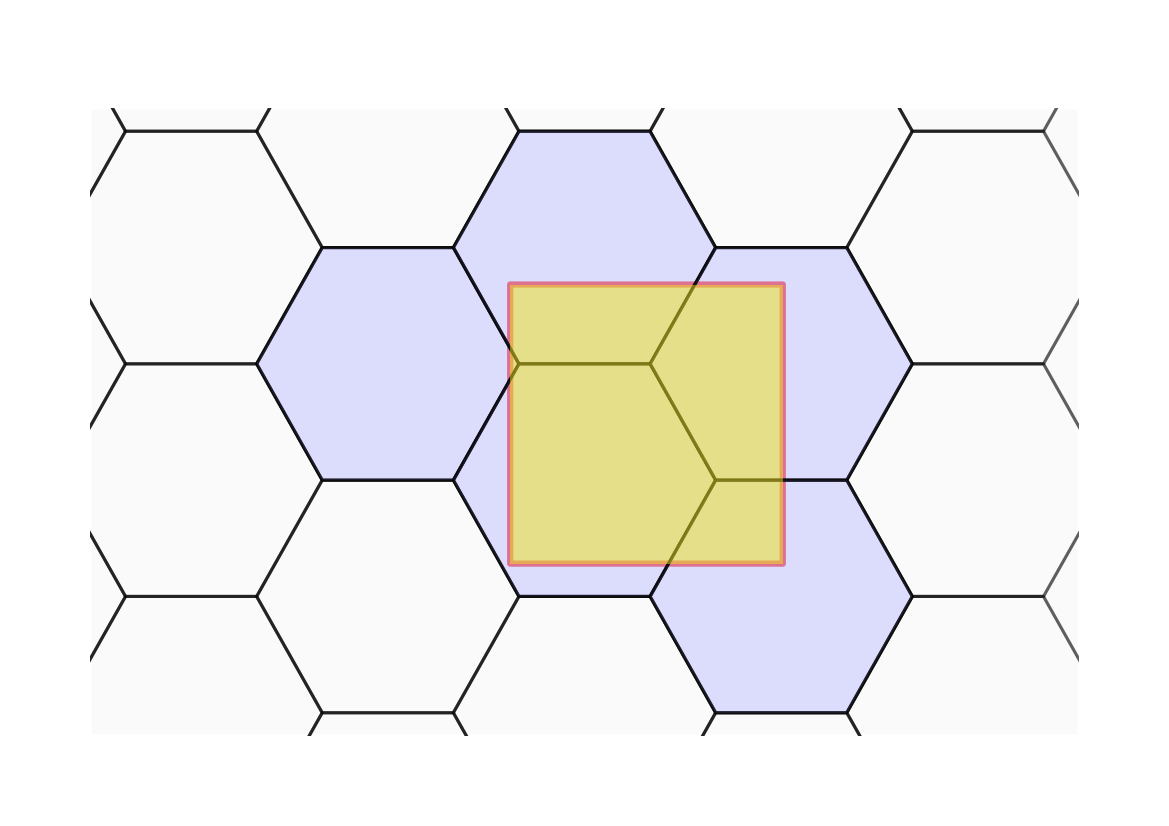
\includegraphics[trim=20 25 20 25, clip, width=.3\textwidth]{fig1a.png}}
    \subcaptionbox{\label{fig:fig1b}}[.33\textwidth]
    {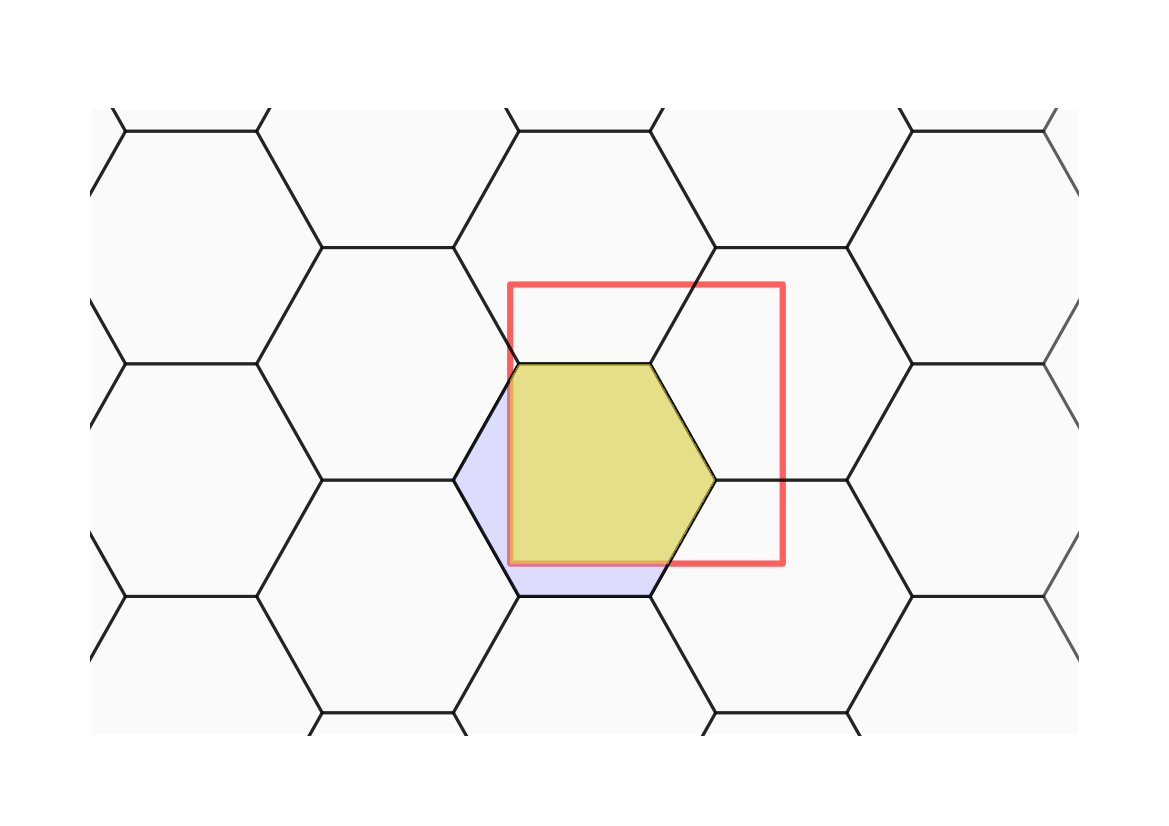
\includegraphics[trim=20 25 20 25, clip, width=.3\textwidth]{fig1b.png}}
    \subcaptionbox{\label{fig:fig1c}}[.33\textwidth]
    {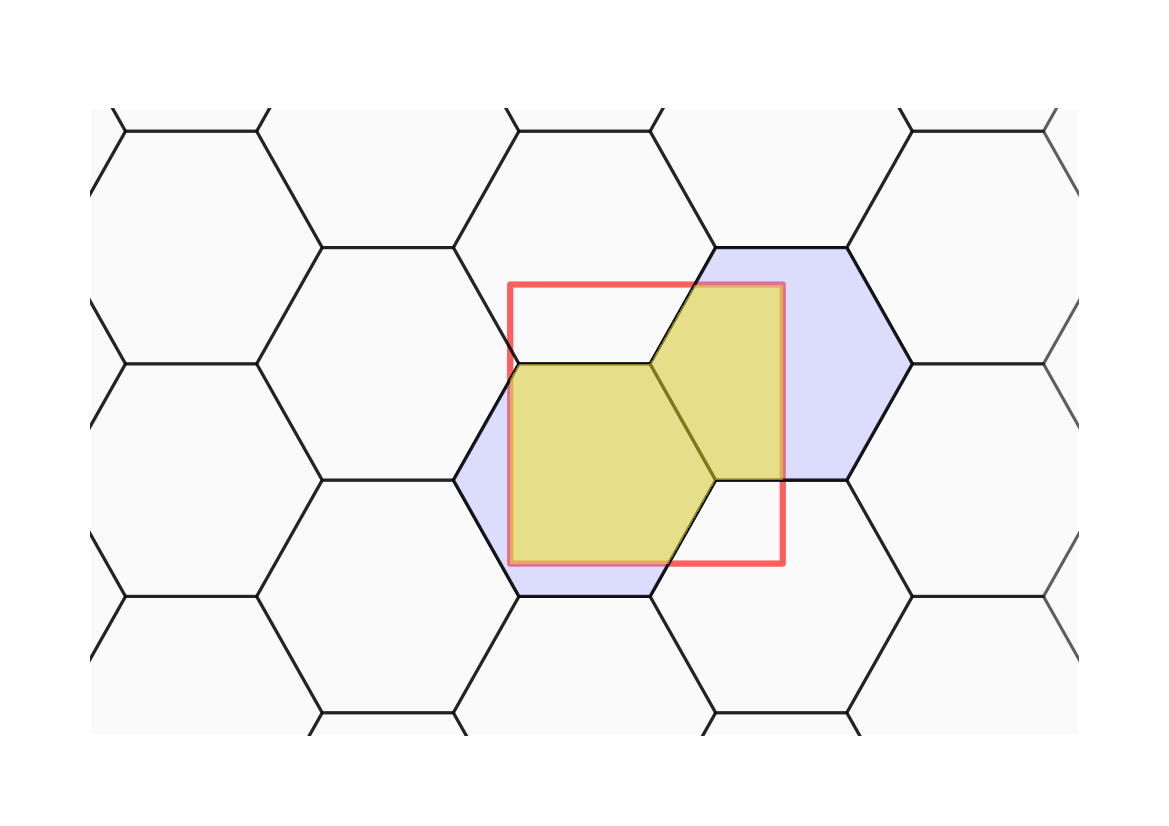
\includegraphics[trim=20 25 20 25, clip, width=.3\textwidth]{fig1c.png}}
    \\
    \subcaptionbox{\label{fig:fig1d}}[.33\textwidth]
    {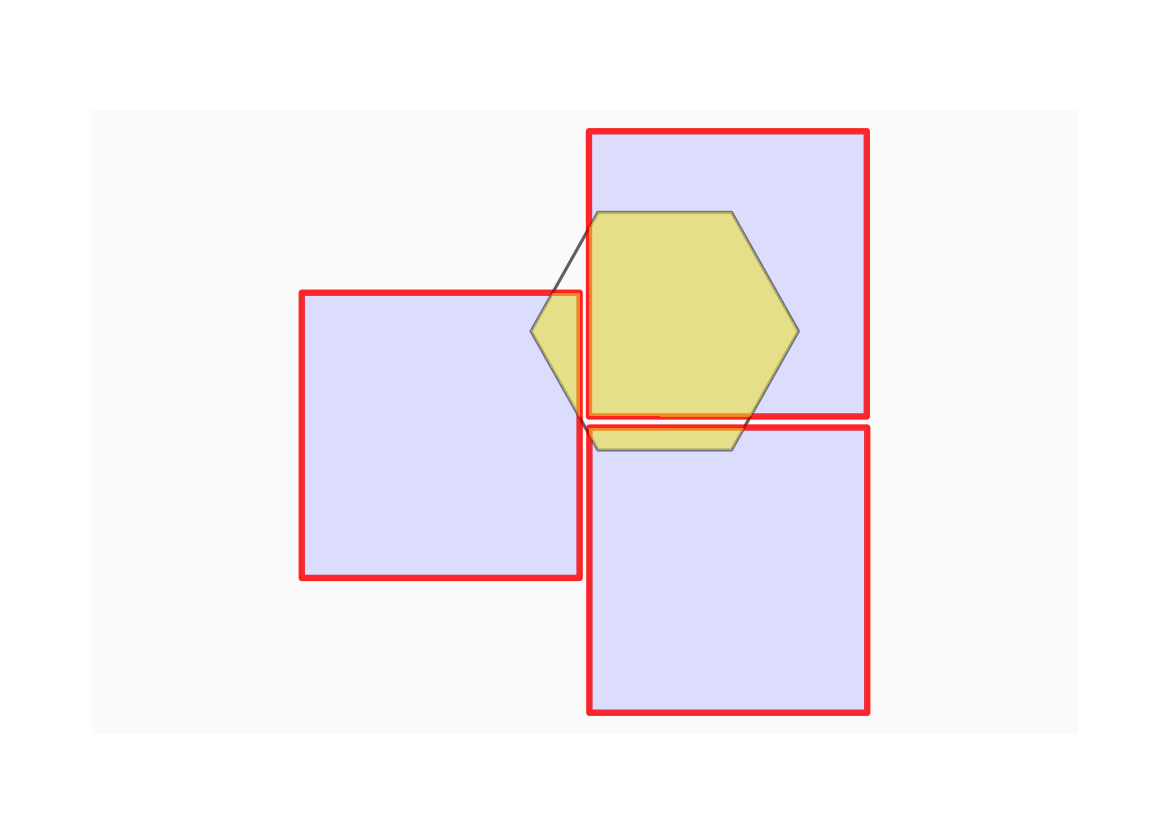
\includegraphics[trim=20 25 20 25, clip, width=.3\textwidth]{fig1d.png}}
    \subcaptionbox{\label{fig:fig1e}}[.33\textwidth]
    {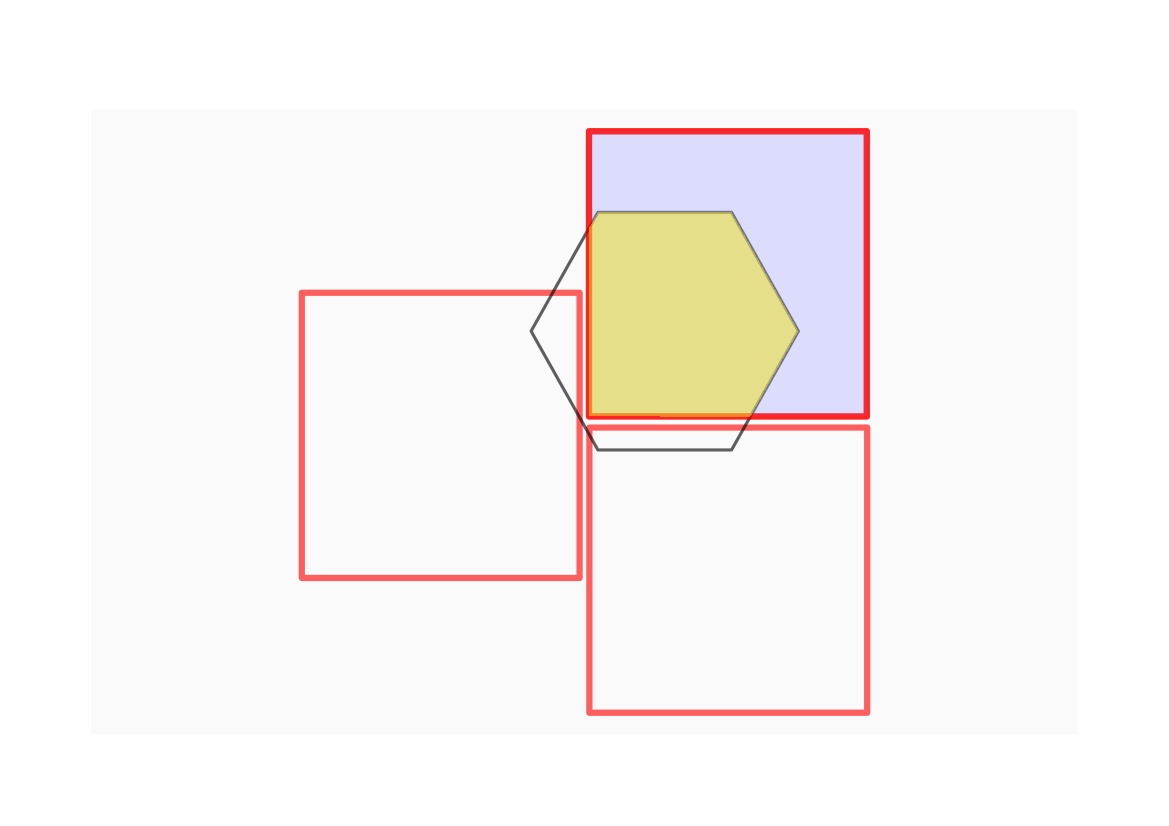
\includegraphics[trim=20 25 20 25, clip, width=.3\textwidth]{fig1e.png}}
    \caption{Subsets are used to compute segmentation metrics. The red squares and black hexagons represent reference and segmented polygons, respectively. (a) $\tilde{Y}$ is made of segmentation polygons overlapping any reference polygon. (b) $Y'$ is made of the segmentation polygon overlapping the most of a reference polygon. (c) ${Y}^{*}$ is made of polygons in the segmentation that either their centroids fall inside the reference, or they cover or overlap more than half of the reference polygon, or the reference polygon centroid falls inside them. (d) $\tilde{X}$ is made of the reference polygons overlapping any segmentation polygon. (e) $X'$ is made of the reference polygons, which overlap the most with the segmentation polygons. Yellow represents the intersection between the references and segments included in a subset. The magenta areas are excluded from the reference-segmentation intersection but included in the subset. Adapted from~\citet{Jozdani2020}.}
    \label{fig:subsets}
\end{figure}

\begin{table}[htbp]
%NOTE: We changed the extrarowheight parameter. The original is 15pt.
\setlength\extrarowheight{10pt}
\centering
\caption{Metrics implemented}
\label{tab:metrics}
\small
\begin{tabular}{lccl}
\toprule
Metric   &  Range  &  Opt.  &  References \\
\midrule
 $\rm{OS1}_{ij}=1-\frac{area(x_i\cap y_j)}{area(x_i)},\ y_j\in {Y^*}_i$ & $[0,1]$ & 0 & \citet{Clinton2010}  \\
 $\rm{OS2}_{ij}=1-\frac{area(x_i\cap y_j)}{area(x_i)},\ y_j\in {Y^{'}}_i$ & $[0,1]$ & 0 & \citet{Persello2010}  \\
 $\rm{OS3}_{ij}=1-\frac{area(x_i\cap y_j)}{area(x_i)},\ y_j\in {Ycd}_i$ & $[0,1]$ & 0 & \citet{Yang2014}  \\
 $\rm{US1}_{ij}=1-\frac{area(x_i\cap y_j)}{area(y_i)},\ y_j\in {Y^*}_i$ & $[0,1]$ & 0 & \citet{Clinton2010}  \\
 $\rm{US2}_{ij}=1-\frac{area(x_i\cap y_j)}{area(y_i)},\ y_j\in {Y^{'}}_i$ & $[0,1]$ & 0 & \citet{Persello2010}  \\
 $\rm{US3}_{ij}=1-\frac{area(x_i\cap y_j)}{area(y_i)},\ y_j\in {Ycd}_i$ & $[0,1]$ & 0 & \citet{Yang2014}  \\
 $\rm{AFI}_{ij}=\frac{area(x_i)-area(y_j)}{area(x_i)},\ y_j\in {Y^{'}}_i$ & $(-\infty,1]$ & 0 & \shortstack[l]{\citet{Lucieer2002};\\  \citet{Clinton2010}}  \\
 $\rm{QR}_{ij}=1-\frac{area(x_i\cap y_j)}{area(x_i\cup y_j)},\ y_j\in {Y^*}_i$ & $[0,1]$ & 0 & \shortstack[l]{\citet{Weidner2008};\\ \citet{Clinton2010}}  \\
 $\rm{D}_{ij}=\sqrt{\frac{\rm{OS}_{ij}^2+\rm{US}_{ij}^2}{2}}$ & $[0,1]$ & 0 & \shortstack[l]{\citet{Levine1982}; \\ \citet{Clinton2010}} \\
 $\rm{precision}_{ij}=\frac{area(x_i\cap y_j)}{area(y_i)},\ y_j\in {Y^{'}}_i$ & $[0,1]$ & 1 & \shortstack[l]{\citet{vanRijsbergen1979};\\ \citet{Zhang2015}}  \\
 $\rm{recall}_{ij}=1-\frac{area(x_i\cap y_j)}{area(x_i)},\ y_j\in {Y^{'}}_i$ & $[0,1]$ & 1 & \shortstack[l]{\citet{vanRijsbergen1979};\\ \citet{Zhang2015}}  \\
 $\rm{UMerging}_{ij}=\frac{area(x_i)-area(x_i\cap y_j)}{area(x_i)},\ y_j\in {Y^*}_i$ & $[0,1]$ & 0 & \shortstack[l]{\citet{Levine1982};\\ \citet{Clinton2010}} \\
 $\rm{OMerging}_{ij}=\frac{area(y_j)-area(x_i\cap y_j)}{area(x_i)},\ y_j\in {Y^*}_i$ & $[0,\infty)$ & 0 & \shortstack[l]{\citet{Levine1982};\\ \citet{Clinton2010}}  \\
 $\rm{M}_{ij}=\sqrt{\frac{area(x_i\cap y_j)^2}{area(x_i)area(y_j)}},\ y_j\in Y^{'}_i$ & $[0,1]$ & 1 & \shortstack[l]{\citet{Janssen1995};\\ \citet{Feitosa2010}} \\
 $\rm{E}_{ij}=\frac{area(y_j)-area(x_i\cap y_j)}{area(y_i)}\times 100,\ x_i\in {X^{'}}_j$ & $[0,100]$ & 0 & \citet{Carleer2005} \\
 $\rm{RAsub}_{ij}=\frac{area(x_i\cap y_j)}{area(x_i)},\ y_j\in \tilde{Y}_i$ & $[0,1]$ & 1 & \shortstack[l]{\citet{Moller2007};\\ \citet{Clinton2010}}  \\
 $\rm{RAsuper}_{ij}=\frac{area(x_i\cap y_j)}{area(y_i)},\ y_j\in \tilde{Y}_i$ & $[0,1]$ & 1 & \shortstack[l]{\citet{Moller2007};\\ \citet{Clinton2010}} \\
 $\rm{PI}_{i}=\sum_{j=1}^{m}{\frac{area(x_i\cap y_j)^2}{area(x_i)area(y_i)}},\ y_j\in \tilde{Y}_i$ & $[0,1]$ & 1 & \citet{VanCoillie2008} \\
 $\rm{Fitness}_{ij}=\frac{area(x_i)+area(y_i) - 2 \times area(x_i\cap y_j)}{area(y_i)},\ x_i\in X^{'}_i$ & $[0,\infty)$ & 0 & \citet{Costa2008} \\
 $\rm{ED3}_{ij}=\sqrt{\frac{OS3_{ij}^2+US3_{ij}^2)}{2}}$ & $[0,1]$ & 0 & \citet{Yang2014} \\
 $\rm{F{\text -}measure}_{ij}$*=$\frac{1}{\frac{\alpha}{\rm{precision}}+\frac{(1-\alpha)}{\rm{recall}}}$ & $[0,1]$ & 1 & \shortstack[l]{\citet{vanRijsbergen1979};\\\citet{Zhang2015}} \\
 $\rm{IoU}_{ij}=\frac{area(x_i\cap y_j)}{area(x_i\cup y_j)},\ y_j\in {Y^{'}}_i$ & $[0,1]$ & 1 & \shortstack[l]{\citet{Jaccard1912};\\\citet{Rezatofighi2019}} \\
 $\rm{SimSize}_{ij}=\frac{min(area(x_i),area(y_j))}{min(area(x_i),area(y_j))},\ y_j\in {Y^*}_i$ & $[0,1]$ & 1 & \shortstack[l]{\citet{Zhan2005}} \\
 $\rm{qLoc}_{ij}=dist(centroid(x_i),centroid(y_j)),\ y_j\in {Y^*}_i$ & $[0,\infty)$ & 0 & \shortstack[l]{\citet{Zhan2005}} \\
 $\rm{RPsub}_{ij}=dist(centroid(x_i),centroid(y_j)),\ y_j\in {\tilde{Y}}_i$ & $[0,\infty)$ & 0 & \shortstack[l]{\citet{Moller2007};\\\citet{Clinton2010}} \\
 $\rm{RPsuper}_{ij}=\frac{dist(centroid(x_i),centroid(y_j))}{max_j(dist(centroid(x_i),centroid(y_j)))},\ y_j\in {Y^*}_i$ & $[0,1]$ & 0 & \shortstack[l]{\citet{Moller2007};\\\citet{Clinton2010}} \\
 $\rm{OI2}_{i}=max_j\left(\frac{area(x_i\cap y_j)}{area(x_i)}*\frac{area(x_i\cap y_j)}{area(y_j)}\right),\ y_j\in {\tilde{Y}}_i$ & $[0,1]$ & 1 & \shortstack[l]{\citet{Yang2017}} \\
 $\rm{Dice}_{i}=\frac{2*area(x_i\cap y_j)}{area(x_i)+area(y_j)},\ y_j\in {Y^{'}}_i$ & $[0,1]$ & 1 & \shortstack[l]{\citet{Dice1945}} \\
\bottomrule
\end{tabular}
\vspace{1ex}
{\raggedright\footnotesize * It takes the optional weight argument $\alpha\in[0,1]$ (the default is 0.5). \par}
\end{table}

Metrics can be computed either from scratch using subsets or by combining other metrics. 
Examples of metrics using subsets include: Oversegmentation (OS), Undersegmentation (US), Area Fit Index (AFI), Quality Rate (QR), Precision, Recall, Undermerging (UMerging), Overmerging (OMerging), Match (M), Evaluation measure (E), Relative area (RAsub and RAsuper), Purity Index (PI), and Fitness Function (Fitness). 
The metrics computed by combining other metrics include: Index D (D), Euclidean Distance (ED3), and F-measure (F\_measure). Some of these metrics are not intended to be summarized such as Relative position (RPsub and RPsuper). 

\section{The segmetric package}

\subsection{Installation}

The stable release of \CRANpkg{segmetric} package can be installed from CRAN, using:

\begin{example}
install.packages("segmetric")
\end{example}

\subsection{Computing metrics}

\CRANpkg{segmetric} depends on the \CRANpkg{sf} package~\citep{Pebesma2018} to open and manipulate geographic vector data sets.
\CRANpkg{sf} is an implementation of a standard issued by the Open Geospatial Consortium~\citep{OGC2011}, which was further formalized in~\citet{ISO2004}. 
This standard defines a common way to store and access spatial data in the context of geographic information systems.

To start with \CRANpkg{segmetric}, users should create a \code{segmetric} object using \code{sm\_read(ref\_sf, seg\_sf)} passing to it a reference spatial data set and a segmentation spatial data set. The parameters \code{ref\_sf} and \code{seg\_sf} should be either \code{sf} objects or paths to a supported file vector format (e.g., \samp{shapefile}). 

\begin{example}
library(segmetric)

# load example data sets
data("sample_ref_sf", package = "segmetric")
data("sample_seg_sf", package = "segmetric")

# create a segmetric object
m <- sm_read(ref_sf = sample_ref_sf, seg_sf = sample_seg_sf)
\end{example}

To compute a metric, users should run the function \code{sm\_compute(m, metric\_id, ...)}, where \code{m} is a \code{segmetric} object and \code{metric\_id} is the identification of a metric in \CRANpkg{segmetric}. Any extra parameter necessary to compute metrics can be informed using the \code{ellipsis} parameter. The list of available metrics can be obtained using \code{sm\_list\_metrics()} which returns a \code{character} vector listing all registered metrics.

The \code{sm\_compute()} function can compute a set of metrics by passing a vector of values to the \code{metric\_id} parameter or making a sequence of function calls using a \code{pipe} operator. The two examples below produce equivalent results:

\begin{example}
# compute three metrics
sm_compute(m, c("AFI", "OS1", "US1"))

# compute the same three metrics as above
sm_compute(m, "AFI") %>%
  sm_compute("OS1") %>%
  sm_compute("US1")
\end{example}

Most metrics are computed by feature (i.e., by reference or segment). To summarize the values of a set of metrics, users can run the function \code{summary(object, ...)}, which computes aggregated values for the metrics returned by \code{sm\_compute()}.

\begin{example}
# compute three metrics
sm_compute(m, c("AFI", "OS1", "US1")) %>%
  summary()
\end{example}

Once created, a \code{segmetric} object stores in the cache every computed subset. Further subset requests are retrieved from the cache, speeding up the computation.

\subsection{How to extend segmetric}

The \CRANpkg{segmetric} package is extensible by providing functions to implement new metrics. To implement a new metric, users can use \code{sm\_new\_metric()} to create a new metric object and register it using \code{sm\_reg\_metric()} function. Users can type \code{?sm\_reg\_metric()} to find more details on how new metrics can be implemented. The following example implements the Jaccard index~\citep{Jaccard1912}, also known as Intersection over Union (\textit{IoU})~\citep{Rezatofighi2019}, which is defined between 0 and 1 (optimal):

\begin{example}
# register 'IoU' metric
sm_reg_metric(
    metric_id = "IoU",
    entry = sm_new_metric(
        fn = function(m, s, ...) {
            # m is the metric object, s is the subset
            #  for IoU, s is equivalent to sm_yprime(m)
            sm_area(s) / sm_area(sm_subset_union(s))
        },
        fn_subset = sm_yprime,
        name = "Intersection over Union",
        optimal = 1,
        description = "Values from 0 to 1 (optimal)",
        reference = "Jaccard (1912); Rezatofighi et al. (2019)"
    )
)

# describes the 'IoU' metric
sm_desc_metric("IoU")
#> * IoU (Intersection over Union)
#>   Values from 0 to 1 (optimal)
#>   reference: Jaccard (1912); Rezatofighi et al. (2019)
\end{example}

Contributions to the package are welcome at GitHub~\footnote{\url{https://github.com/michellepicoli/segmetric}} and more details on how to contribute can be found in segmetric home-page at \url{https://michellepicoli.github.io/segmetric}.


\section{Package segmetric in action}

The specific steps involved in a segmentation workflow can vary depending on researcher goals, characteristics of the input data, and the task requirements. In general, a segmentation workflow typically includes the steps in Figure~\ref{fig:workflow}. 
First, researchers working with segmentation data need to obtain satellite images and preprocess them via methods such as radiometric and geometric corrections, image mosaicking, cloud masking, indices computation, and texture extraction. 
Second, a segmentation method is used to obtain the segments. Typically, researchers can use supervised and unsupervised machine learning methods such as convolutional neural network~\citep{Fukushima1980}, U-Net~\citep{Ronneberger2015}, multi-resolution segmentation~\citep{Baatz2000}, and watershed segmentation~\citep{Beucher1992}. In this step, the segments can be stored in a vector format.
Finally, the accuracy of the segmentation can be assessed by supervised quality metrics. Using reference data, researchers compute metrics to evaluate the segmentation. 
The last two steps may be repeatedly iterated until the desired level of accuracy is reached.

\begin{figure}[htbp]
  \centering
  \includegraphics[width=1\textwidth]{fig2.png}
  \caption{General steps of segmentation workflow.}
  \label{fig:workflow}
\end{figure}

In the following section, we demonstrate an application of the \CRANpkg{segmetric} package to assess several segmentation parameters and guide users to select the most accurate one.

\subsection{Data}

In agriculture studies, mapping characteristics such as the size and number of fields can provide information about productivity and other important variables such as food security, socioeconomic status, and environmental status. To demonstrate \CRANpkg{segmetric}, we used data on the Luís Eduardo Magalhães (LEM) municipality, west of Bahia state, Brazil. This municipality belongs to the Brazilian agricultural frontier known as MATOPIBA, which includes the states of Maranhão (MA), Tocantins (TO), Piauí (PI), and Bahia (BA) (Figure \ref{fig:studyarea}). 

\begin{figure}[htbp]
  \centering
  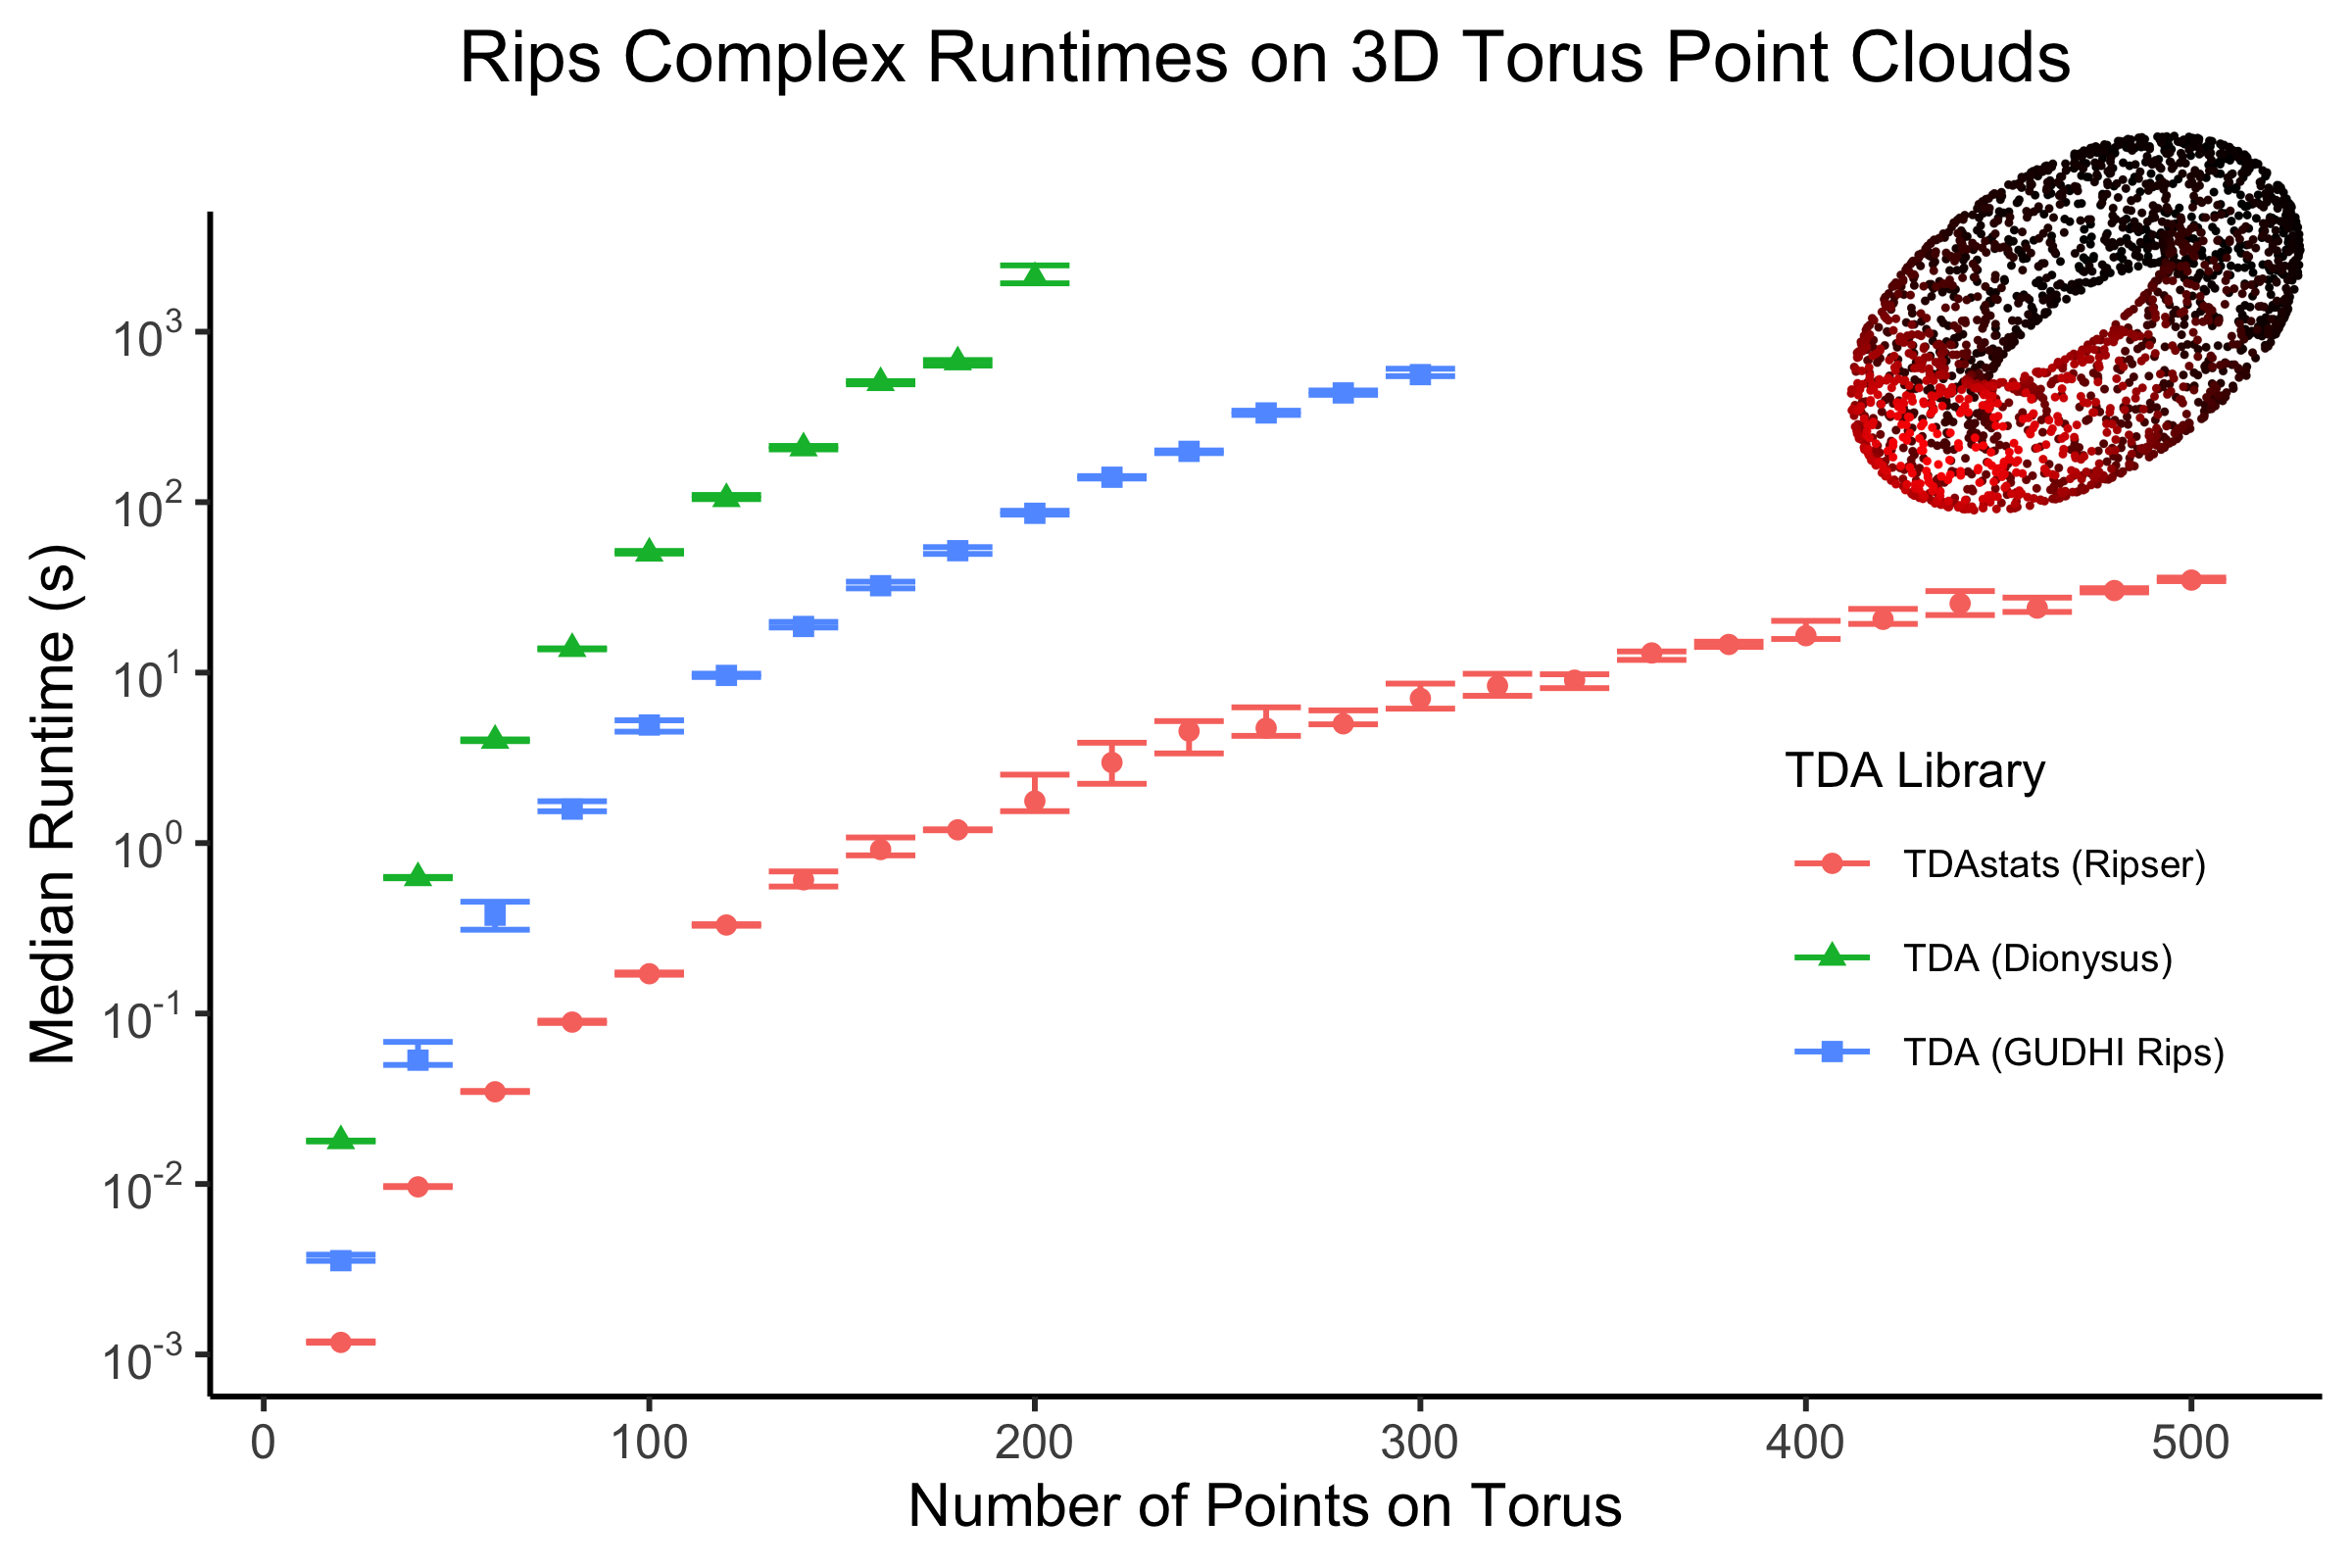
\includegraphics[width=1\textwidth]{fig3.png}
  \caption{Study area in Luís Eduardo Magalhães municipality, west of Bahia state, Brazil (Google Earth imagery). Reference data (in red) was provided by~\citet{Oldoni2020}.}
  \label{fig:studyarea}
\end{figure}

We used three PlanetScope images acquired on Feb 18, 2020, with a 3.7-meter resolution and four spectral bands (blue, green, red, and near-infrared). Radiometric and geometric corrections were applied to the image (level 3B)~\citep{Planet2017}. The images were in the same projection (UTM zone 23S) and we mosaicked them.

We segmented the image applying a multi-resolution segmentation approach~\citep{Baatz2000}. We tested four scale parameters (SP) to segment the image: 200, 500, 800, and 1000; shape parameter: 0.9;  and compactness: 0.1. The resulting polygons were simplified using the Douglas-Peucker algorithm~\citep{Douglas1973} (distance parameter: 10 meters) in QGIS software (version 3.22.2). The Self-intersections were removed using SAGA's Polygon Self-Intersection tool (version 7.8.2). The final segmentation set is composed of polygons intersecting the reference data with an area-perimeter ratio above 25. 
The segmentation results are provided as part of the \CRANpkg{segmetric} package.

The reference data set (ref\_sf), provided by \citet{Oldoni2020}, was collected in two fieldwork campaigns in March and August 2020. \citet{Oldoni2020} draw the field boundaries in-situ on top of images Sentinel-2, with a spatial resolution of 10 meters. \CRANpkg{segmetric} includes only a portion of this data set. The spatial data sets can be loaded into R using \CRANpkg{sf} objects. To create a \CRANpkg{segmetric} object, use function \code{sm\_read()}:

\begin{example}
library(segmetric)

# load data sets
data("ref_sf", package = "segmetric")
data("seg200_sf", package = "segmetric")
data("seg500_sf", package = "segmetric")
data("seg800_sf", package = "segmetric")
data("seg1000_sf", package = "segmetric")

# create a segmetric object
m200 <- sm_read(ref_sf = ref_sf, seg_sf = seg200_sf)
m500 <- sm_read(ref_sf = ref_sf, seg_sf = seg500_sf)
m800 <- sm_read(ref_sf = ref_sf, seg_sf = seg800_sf)
m1000 <- sm_read(ref_sf = ref_sf, seg_sf = seg1000_sf)
\end{example}

\subsection{Analysis}

This analysis assesses four different segmentations with different Scale Parameters (SP) to verify which one fits better with the reference polygons. First, we visualize the reference polygons and the four segmentations individually using the plot() function (Figure \ref{fig:plot}). 

\begin{example}
# plot layers
plot(m200, layers = "ref_sf", plot_centroids = FALSE) 
plot(m200, layers = "seg_sf", plot_centroids = FALSE) 
plot(m500, layers = "seg_sf", plot_centroids = FALSE) 
plot(m800, layers = "seg_sf", plot_centroids = FALSE) 
plot(m1000, layers = "seg_sf", plot_centroids = FALSE)
\end{example}

\begin{figure}[htb]
    \subcaptionbox{\label{fig:fig4a}}[.33\textwidth]
    {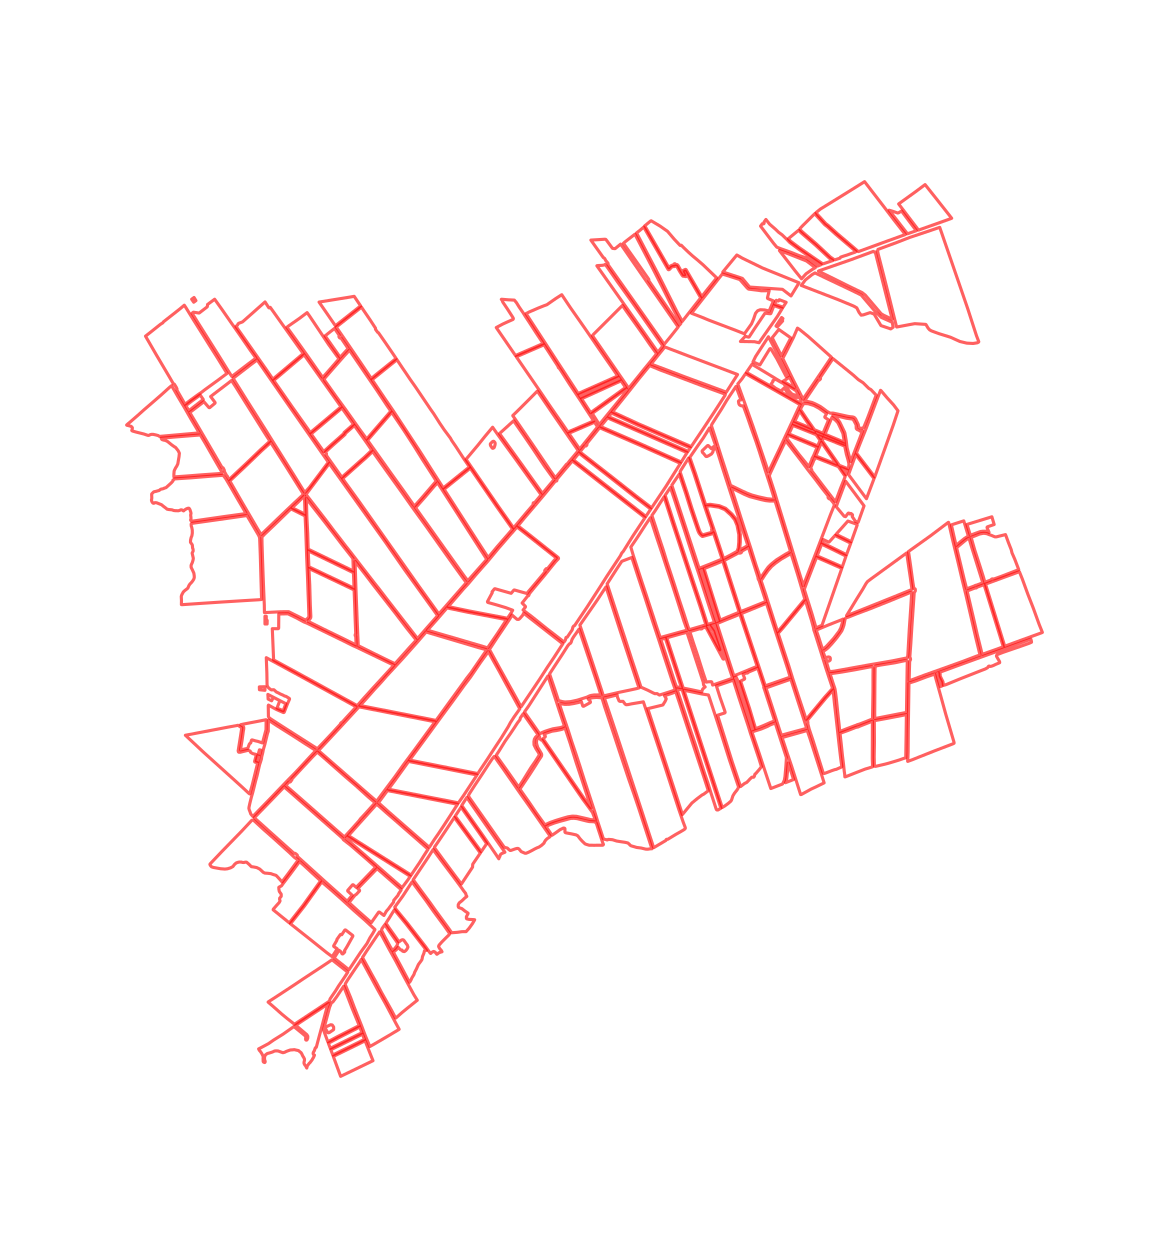
\includegraphics[trim=20 25 20 25, clip, width=.33\textwidth]{fig4a.png}}
    \subcaptionbox{\label{fig:fig4b}}[.33\textwidth]
    {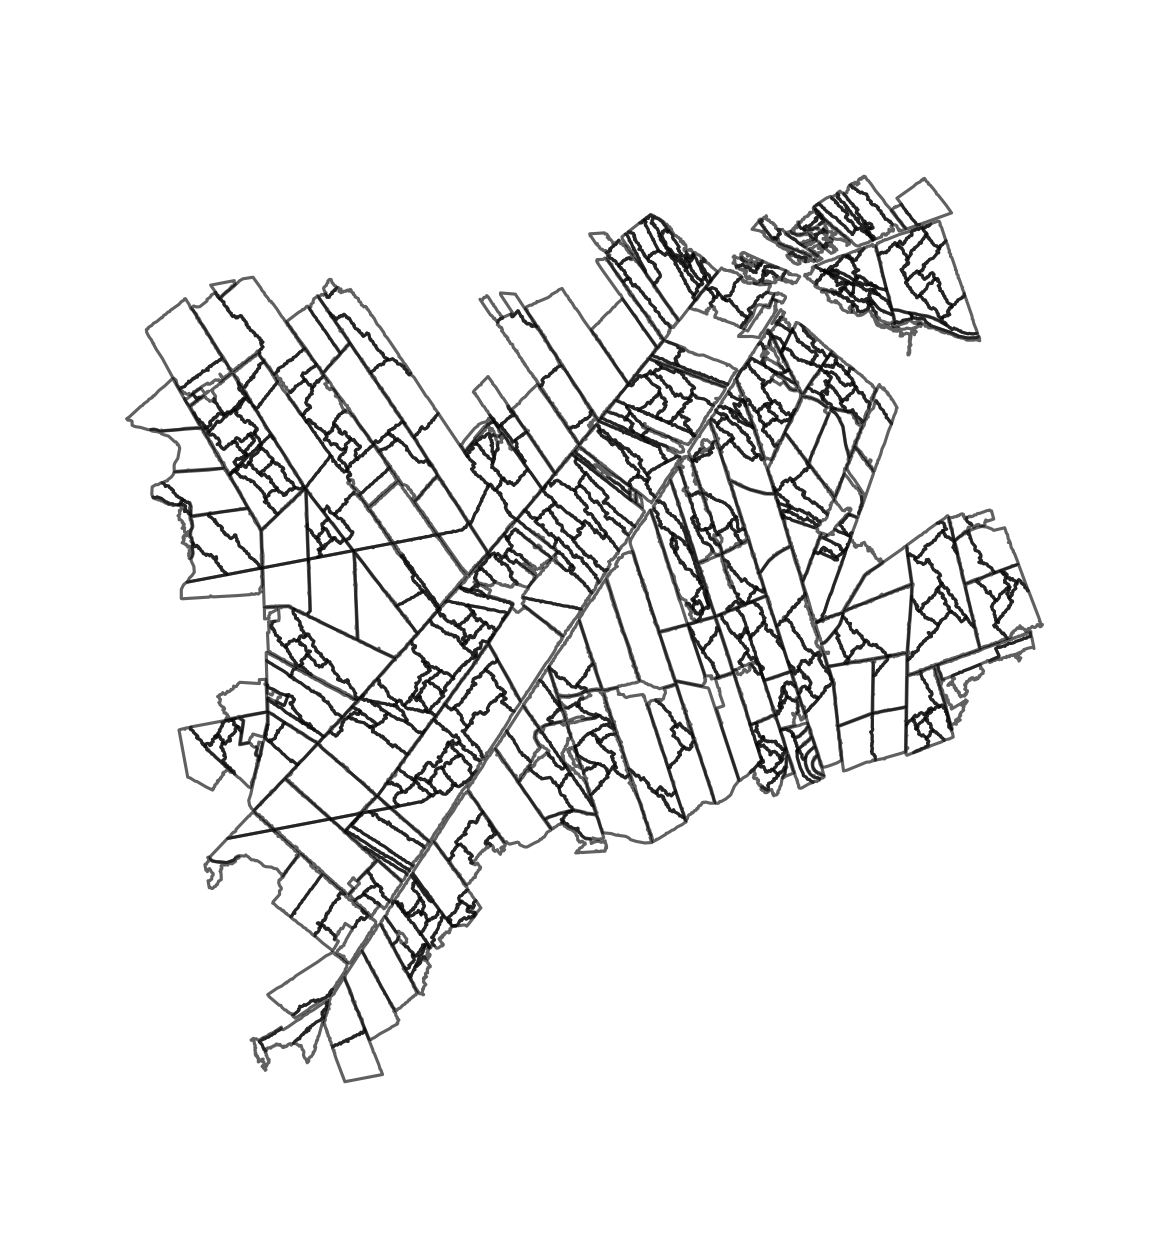
\includegraphics[trim=20 25 20 25, clip, width=.33\textwidth]{fig4b.png}}
    \subcaptionbox{\label{fig:fig4c}}[.33\textwidth]
    {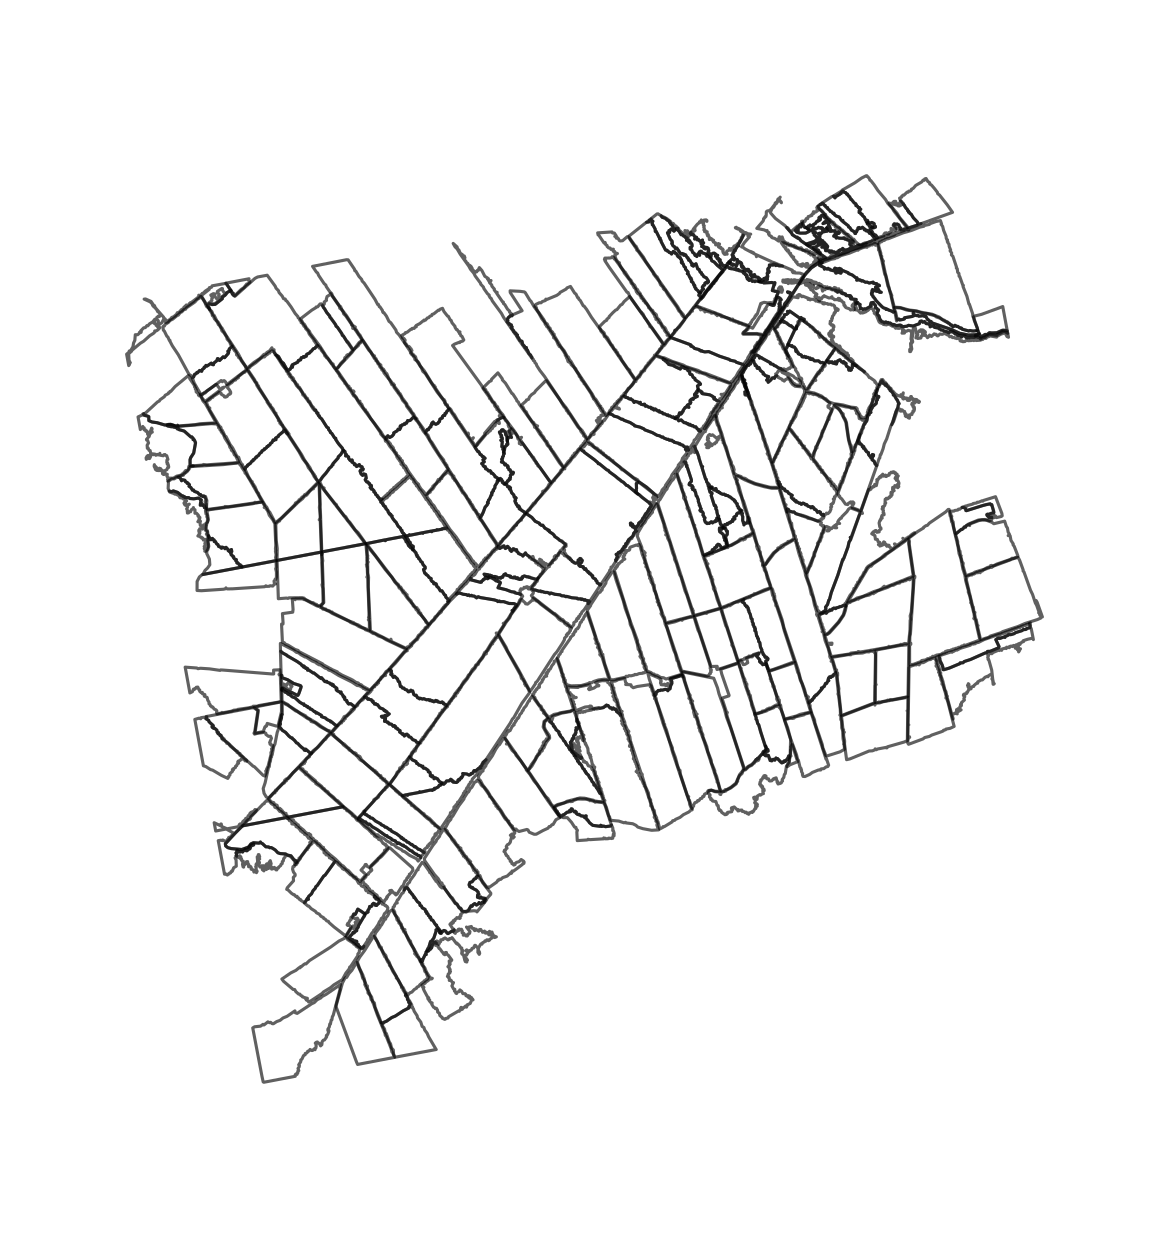
\includegraphics[trim=20 25 20 25, clip, width=.33\textwidth]{fig4c.png}}
    \\
    \subcaptionbox{\label{fig:fig4d}}[.33\textwidth]
    {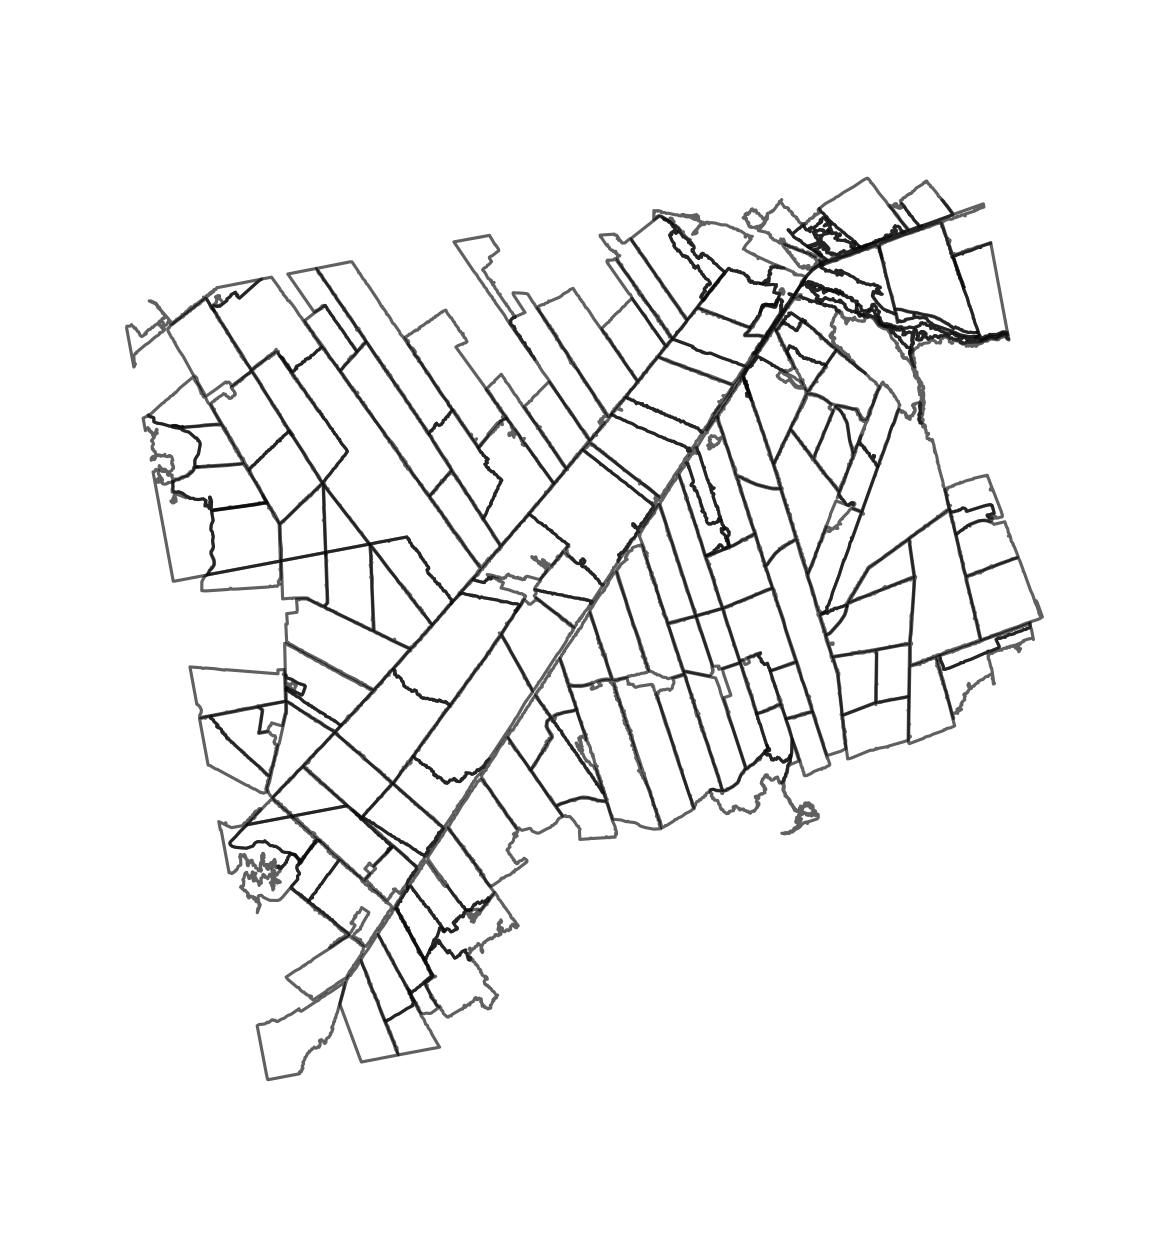
\includegraphics[trim=20 25 20 25, clip, width=.33\textwidth]{fig4d.png}}
    \subcaptionbox{\label{fig:fig4e}}[.33\textwidth]
    {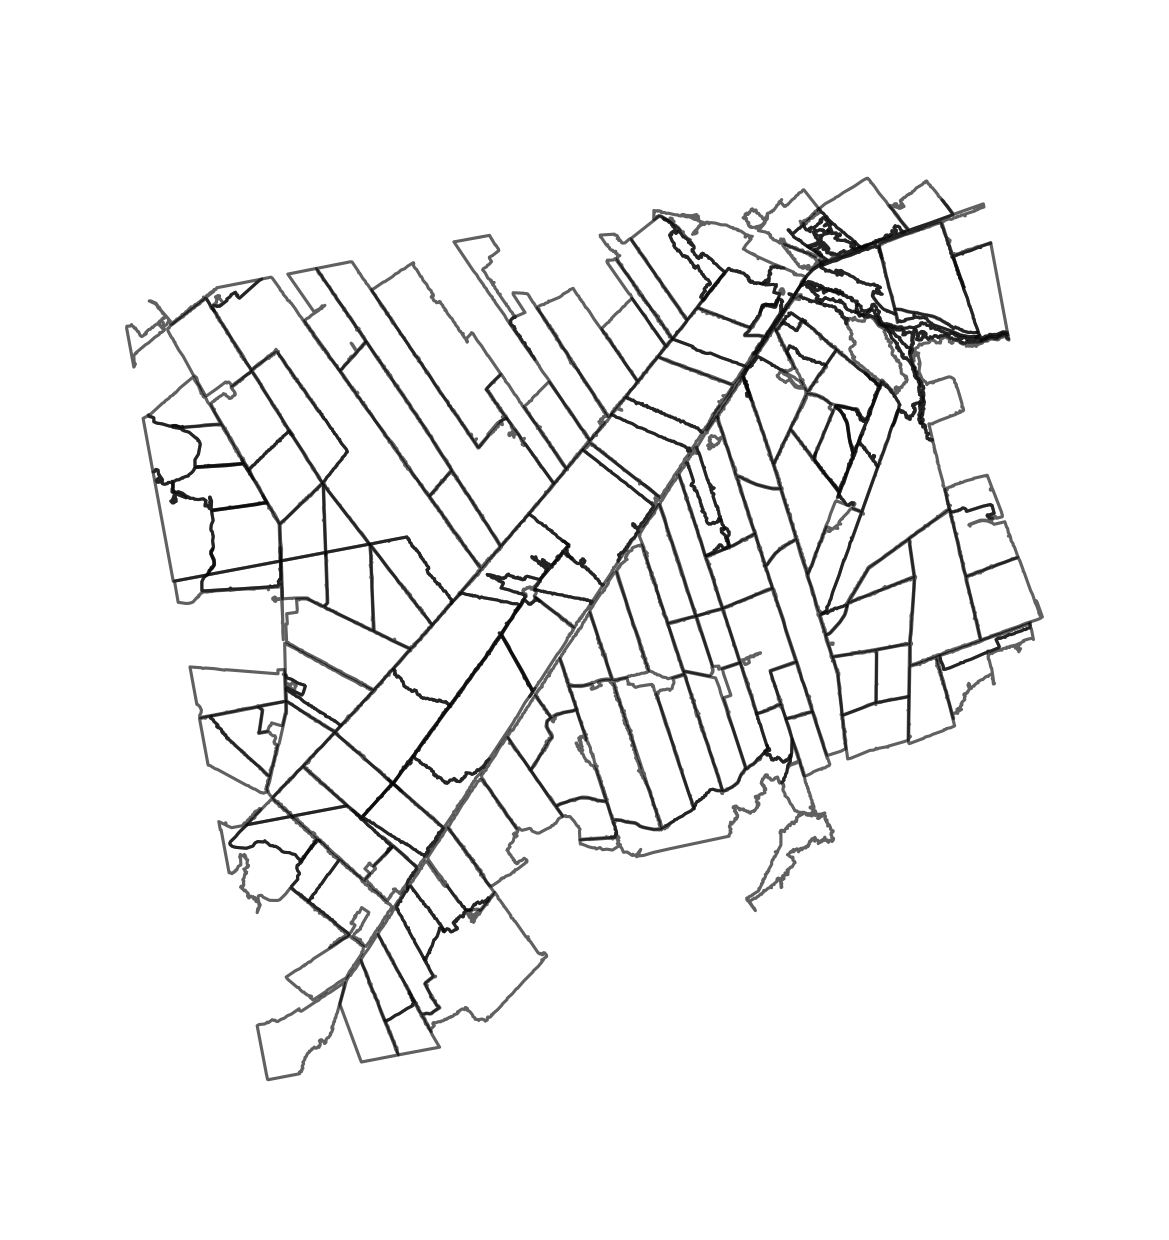
\includegraphics[trim=20 25 20 25, clip, width=.33\textwidth]{fig4e.png}}
    \caption{(a) reference polygons; (b) segmentation using  SP = 200; (c) segmentation using  SP = 500; (d) segmentation using  SP = 800; (e) segmentation using  SP = 1000.}
    \label{fig:plot}
\end{figure}

The metrics available in the package can be consulted using the function \code{sm\_list\_metrics()}. In this example, the metrics chosen to evaluate the accuracy of the segmentations and verify the best value of the scale parameter were: Area Fit Index ~\citep{Carleer2005}, F-measure~ \citep{vanRijsbergen1979} \citep{Zhang2015},  Quality Rate ~\citep{Weidner2008} \citep{Clinton2010}, Oversegmentation ~\citep{Clinton2010}, and Undersegmentation ~\citep{Clinton2010}.

\begin{example}
# compute all metrics
metrics <- c("QR", "F_measure", "IoU", "M", "OS2", "US2")
m200 <- sm_compute(m200, metrics)
m500 <- sm_compute(m500, metrics)
m800 <- sm_compute(m800, metrics)
m1000 <- sm_compute(m1000, metrics)

# results
summary(m200)
#>        QR F_measure       IoU         M       OS2       US2
#> 0.7394817 0.6988555 0.4988198 0.6569973 0.2948025 0.2585708

summary(m500)
#>         QR  F_measure        IoU          M        OS2        US2 
#> 0.50380348 0.80671198 0.56837519 0.70140431 0.07982693 0.37207120 

summary(m800)
#>         QR  F_measure        IoU          M        OS2        US2 
#> 0.47487615 0.78764418 0.54923433 0.68297970 0.04300207 0.43014287 


summary(m1000)
#>         QR  F_measure        IoU          M        OS2        US2 
#> 0.50311268 0.75742922 0.51745883 0.65548524 0.03679037 0.46524463 
\end{example}

The computed metrics are presented in Table \ref{tab:result}; the optimal value of QR, OS2, and US2 is 0, and 1 for F-measure, M, and IoU. These results indicate that segmentation using SP equal to 200 had the highest oversegmentation while using SP equal to 1000 had the highest undersegmentation. Observing the metrics F-measure, IoU, and M, we conclude that the best SP is 500.

Users must pay attention to which metric better fits their goals of accuracy assessment. For more information, we suggest the user consult comparative studies dedicated to geometric metrics such as \citet{Clinton2010}, \citet{Rasanen2013}, \citet{Yang2015}, \citet{Costa2018}, and \citet{Jozdani2020}.


\begin{table}[htbp]
\caption{Accuracy metrics of Quality Rate (QR), F-measure, Intersection over Union (IoU), Match (M), Oversegmentation (OS2), and Undersegmentation (US2) for four segmentations with different Scale Parameters (SP).}
\centering
\small
\begin{tabular}{lllllll}
\toprule
 & \multicolumn{1}{c}{\textbf{QR}} & \multicolumn{1}{c}{\textbf{F\_measure}} & \multicolumn{1}{c}{\textbf{IoU}} & \multicolumn{1}{c}{\textbf{M}} & \multicolumn{1}{c}{\textbf{OS2}} & \multicolumn{1}{c}{\textbf{US2}} \\ \midrule
seg 200 & 0.739 & 0.699 & 0.499 & 0.657 & 0.295 & 0.259 \\
seg 500 & 0.504 & 0.807 & 0.568 & 0.701 & 0.080 & 0.372 \\
seg 800 & 0.475 & 0.788 & 0.549 & 0.683 & 0.043 & 0.430 \\
seg 1000 & 0.503 & 0.757 & 0.517 & 0.655 & 0.037 & 0.465 \\
\bottomrule
\end{tabular}
\label{tab:result}
\end{table}

The \CRANpkg{segmetric} package allows users to visualize subsets used to compute metrics. The example in Figure \ref{fig:ref_seg} shows the results of the function to plot the subset \code{Y\_tilde} over the reference and the segmentation polygons (SP = 500). This allows analyzing the overlap between the reference and segmentation polygons visually.

\begin{example}


plot(
    x = m500, 
    type = "subset", 
    subset_id = "Y_tilde", 
    plot_centroids = FALSE, 
    plot_legend = TRUE, 
    extent = sm_seg(m500) 
)
\end{example}

\begin{figure}[ht]
  \centering
  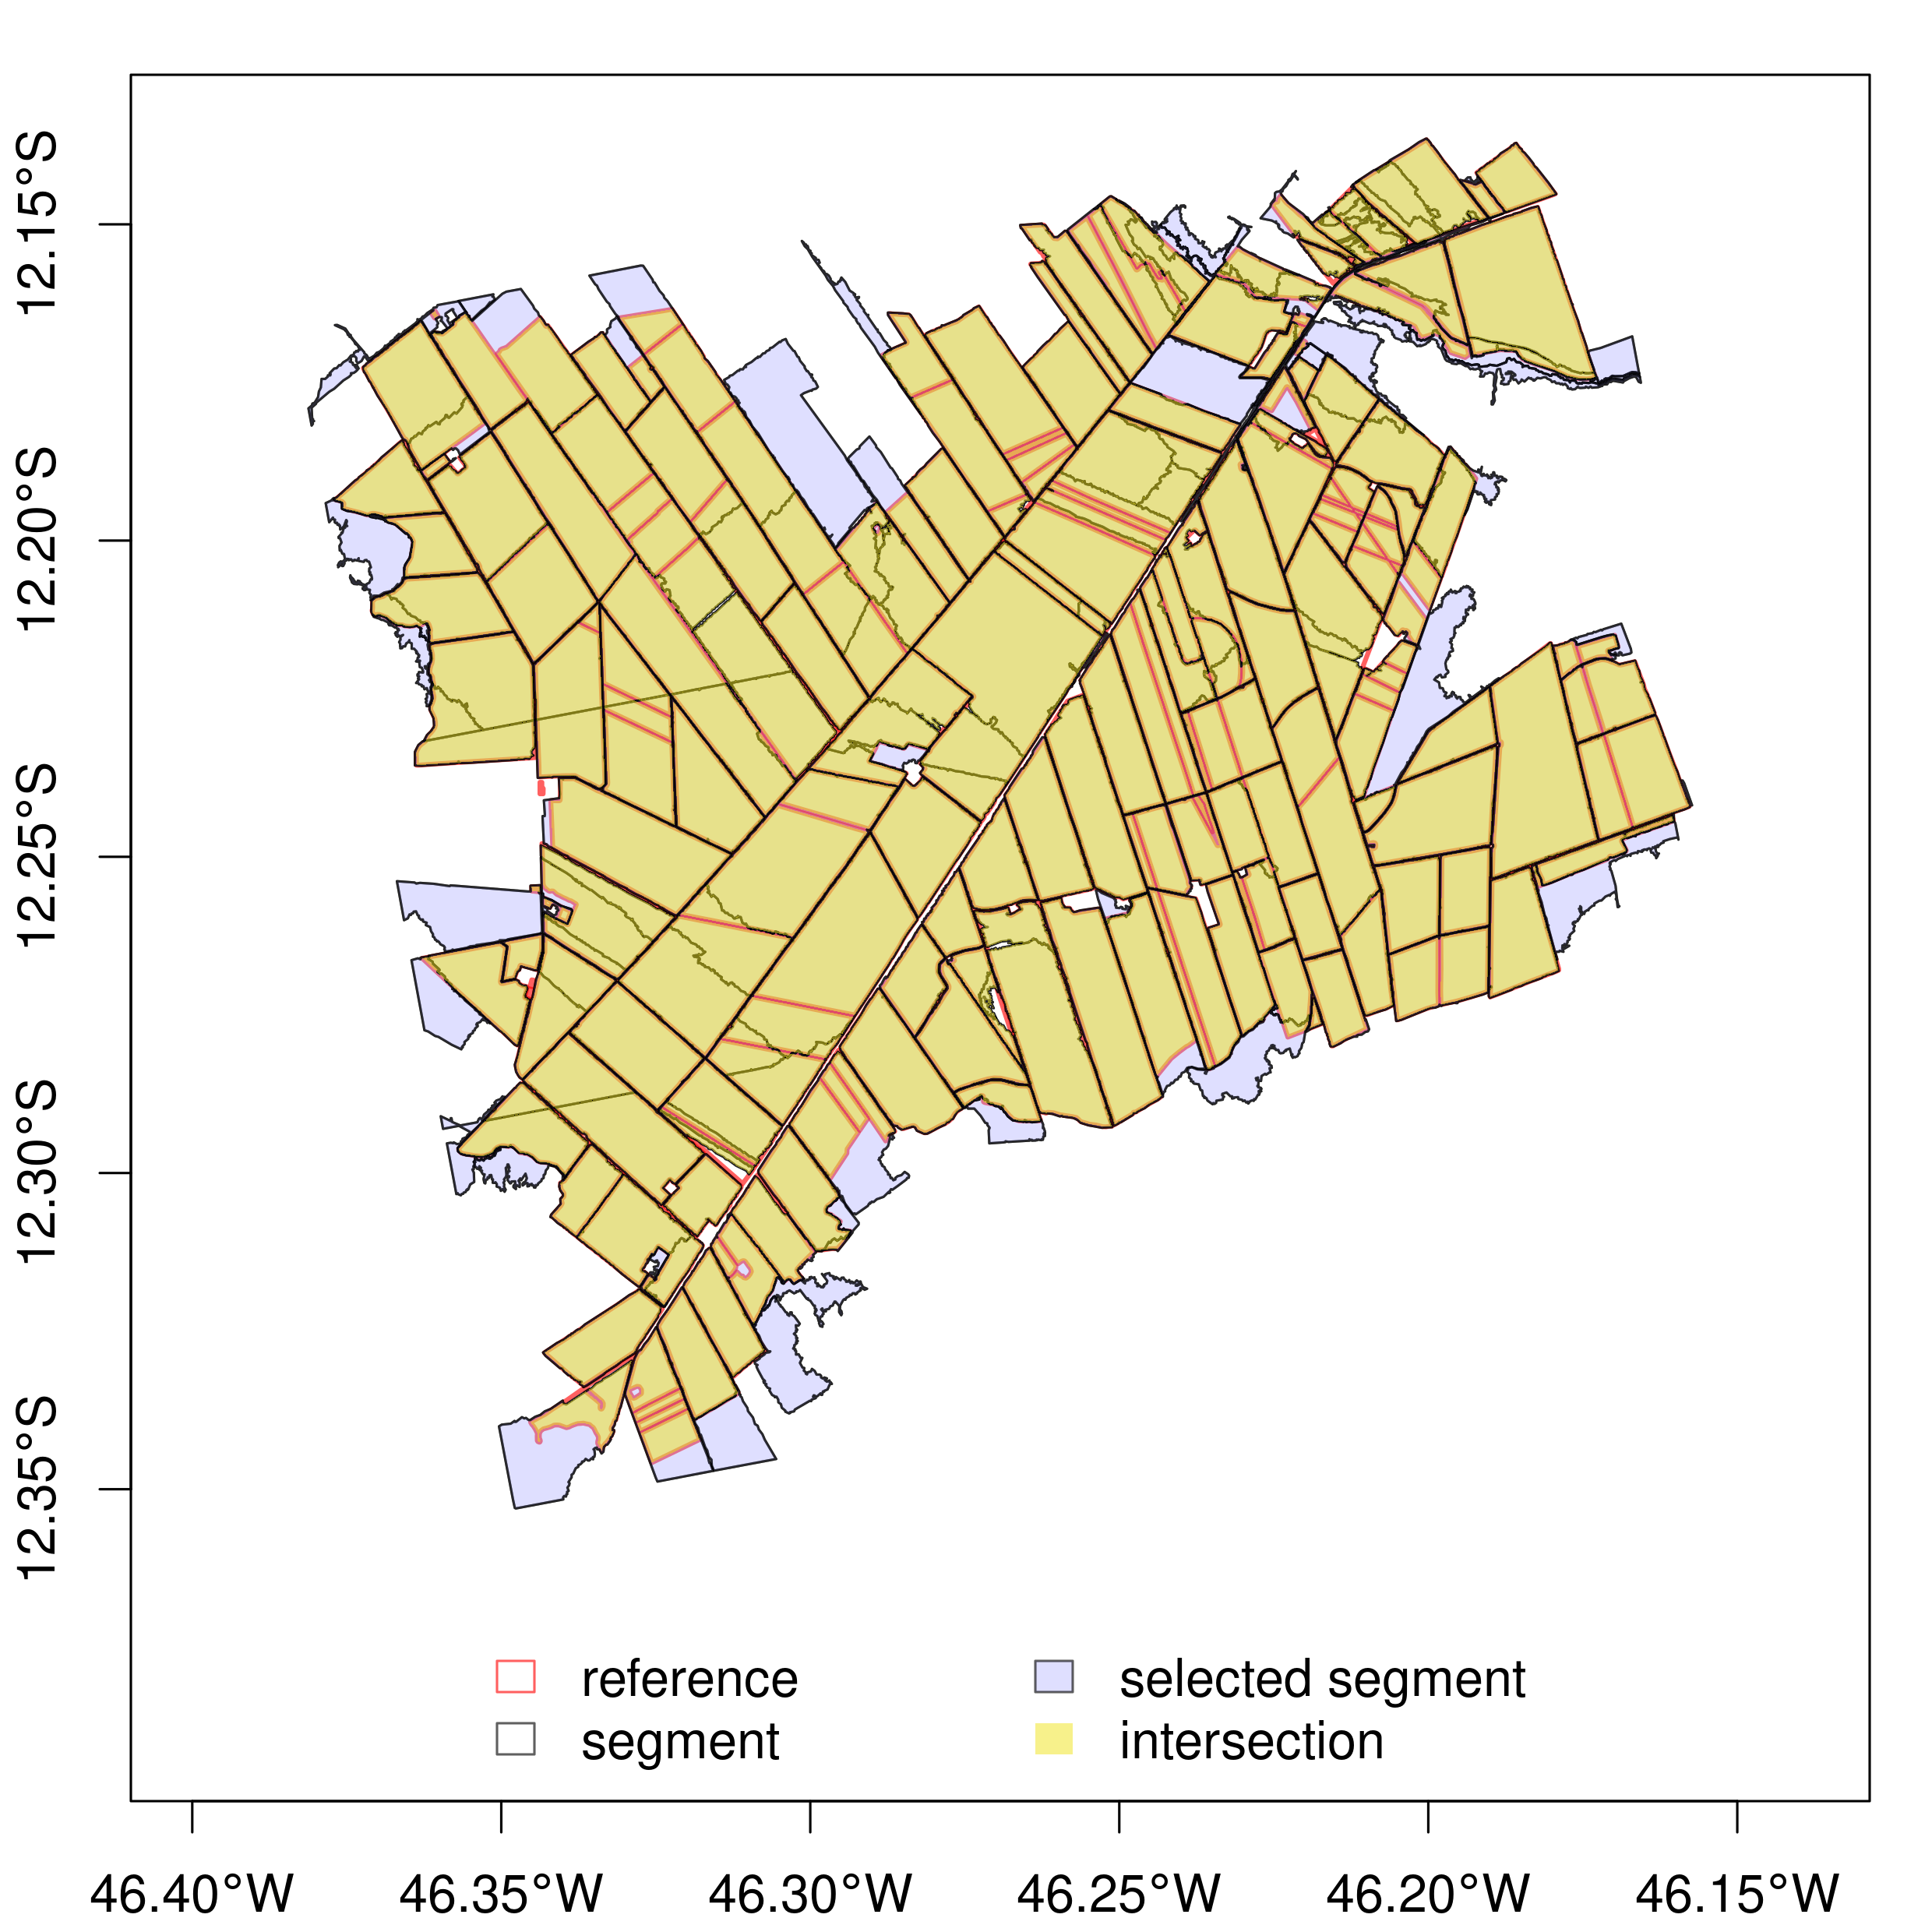
\includegraphics[width=0.7\textwidth]{fig5.png}
  \caption{Overlapping between reference polygons and segmentation objects (SP = 500).}
  \label{fig:ref_seg}
\end{figure}

It is also possible to visualize the metrics for each segment in choropleth maps using the function:

\begin{example}
plot(
    x = m500,
    type = "choropleth",
    metric_id = c("QR", "IoU", "M", "OS2", "US2"),
    break_style = "jenks",
    choropleth_palette = "RdYlBu",
    plot_centroids = FALSE
)
\end{example}

Legend bar of choropleth maps are generated automatically, and users can further customize it with options such as the number of breaks and the palette.
The legend consistently uses the same color for the optimal metric value (for example, in Figure~\ref{fig:plot_metrics}, blue is better while red is worse), except for those metrics in which the optimal value is in the middle of the color scale (e.g., AFI). 
The size and number of intervals in each color scale change accordingly to the metric values present in the data set. 
Users can choose the method to compute the intervals. 
To check available options use \code{?plot.segmetric} and see \code{break\_style} parameter.

\begin{figure}[!ht]
    \subcaptionbox{\label{fig:fig6a}}[.49\textwidth]
    {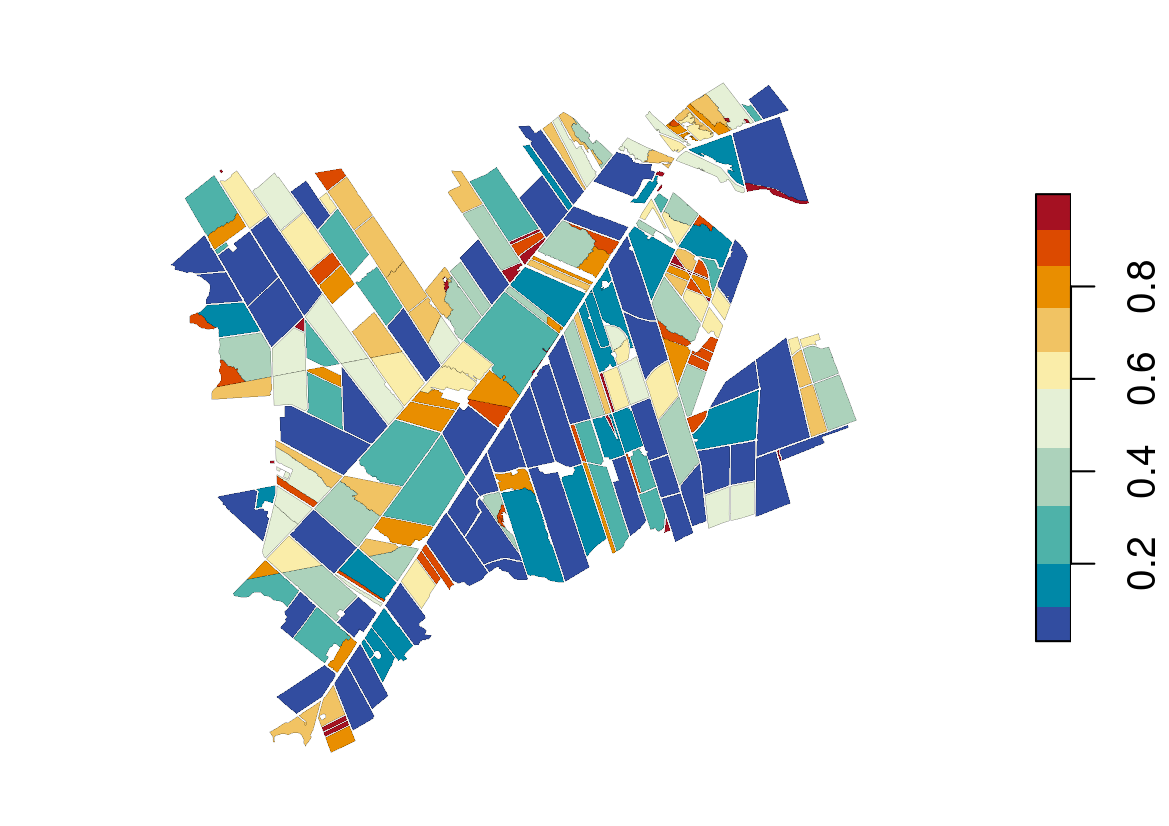
\includegraphics[trim=60 10 0 10, clip, width=.49\textwidth]{fig6a.png}}
    \subcaptionbox{\label{fig:fig6b}}[.49\textwidth]
    {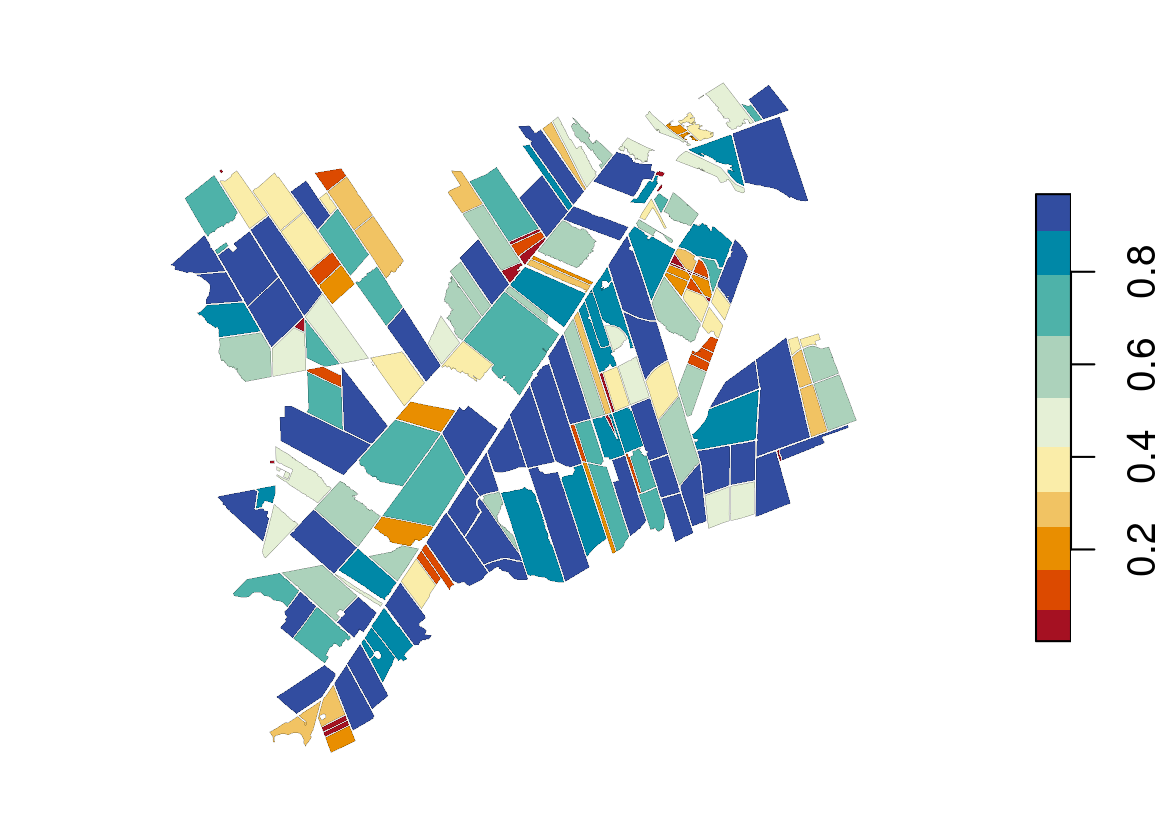
\includegraphics[trim=60 10 0 10, clip, width=.49\textwidth]{fig6b.png}}
    \\
    \subcaptionbox{\label{fig:fig6c}}[.49\textwidth]
    {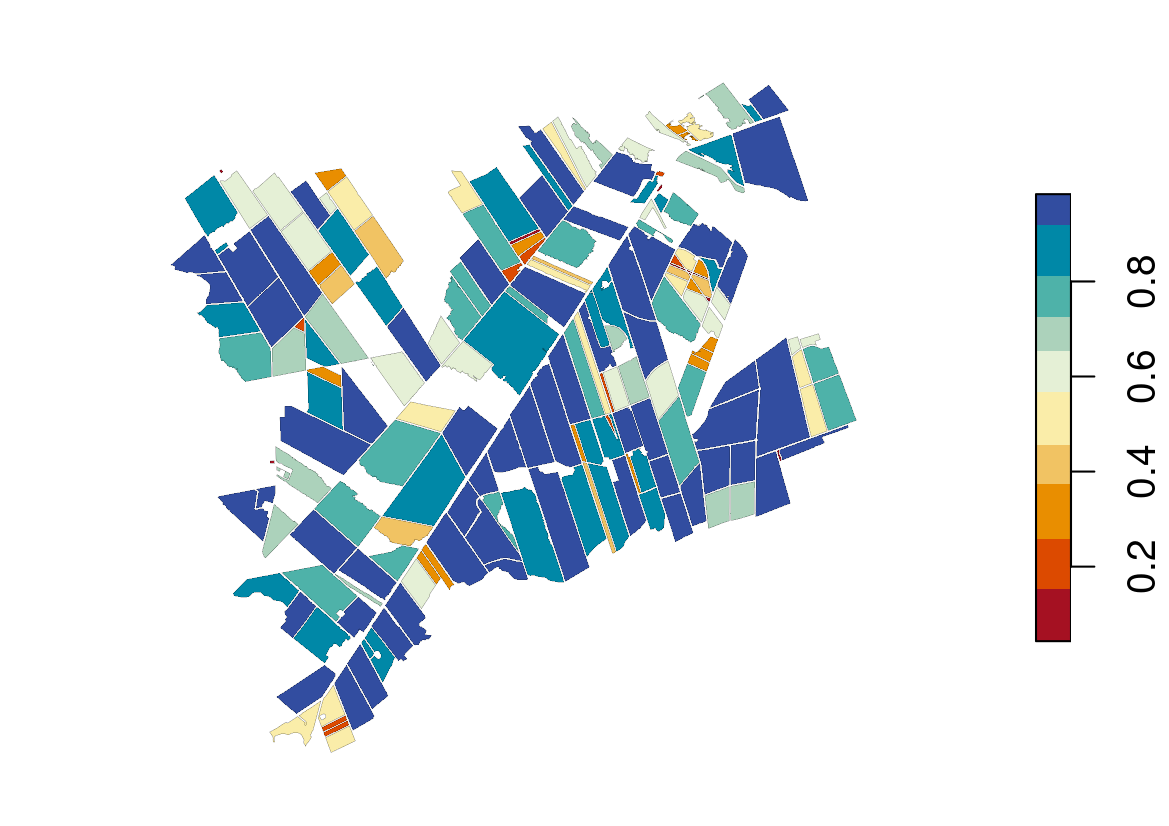
\includegraphics[trim=60 10 0 10, clip, width=.49\textwidth]{fig6c.png}}
    \subcaptionbox{\label{fig:fig6d}}[.49\textwidth]
    {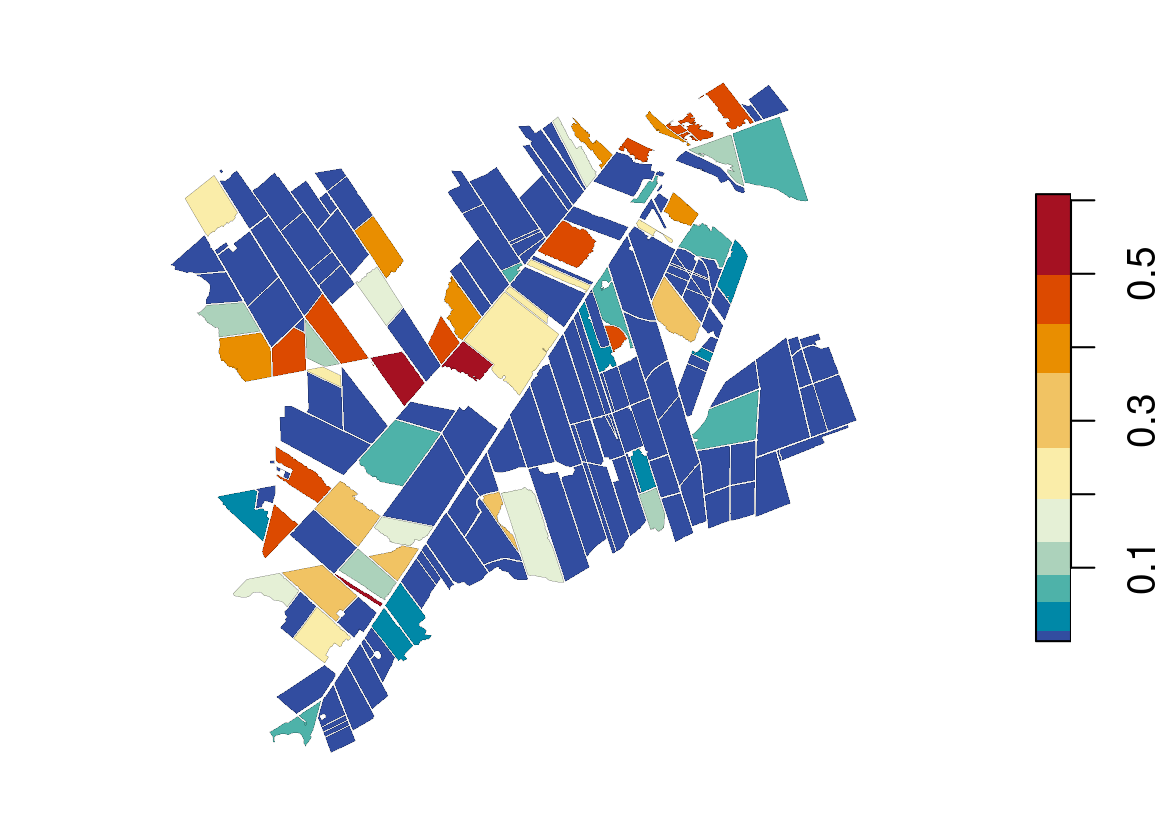
\includegraphics[trim=60 10 0 10, clip, width=.49\textwidth]{fig6d.png}}
    \\
    \subcaptionbox{\label{fig:fig6e}}[.49\textwidth]
    {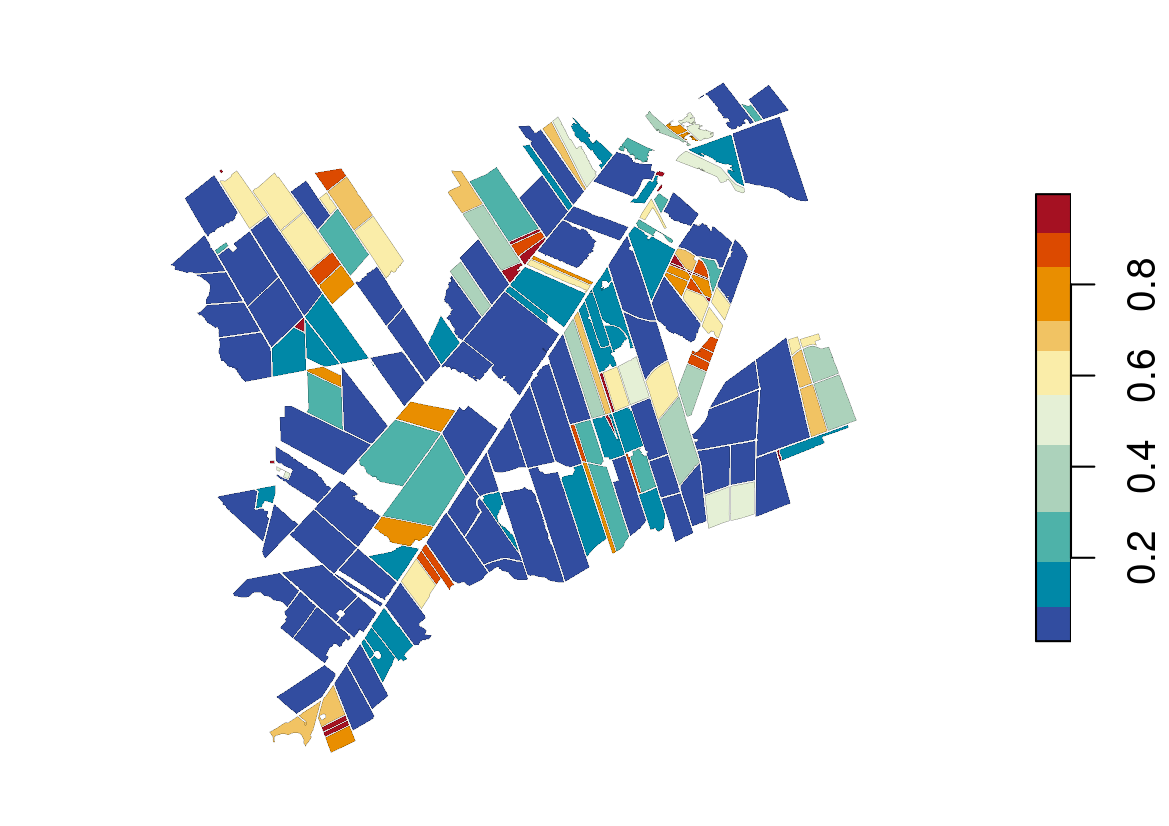
\includegraphics[trim=60 10 0 10, clip, width=.49\textwidth]{fig6e.png}}
    \caption{Spatial distribution of the metrics: (a) Quality Rate, (b) Intersection over Union, (c) Match, (d) Oversegmentation, and (e) Undersegmentation.}
    \label{fig:plot_metrics}
\end{figure}

Figure \ref{fig:plot_metrics} presents the spatialized results of the calculated metrics. 
The F-measure metric was not plotted because it is a global metric with a single value for all objects. 
Figures \ref{fig:plot_metrics}a, d, and e show the similarity between the QR, OS, and US metrics results, for which the ideal value is zero. 
In the three plots of these metrics, it is noted that the objects with the best results (close to zero) are located in the southeast part of the study area.
The IoU and M metric maps (Figure \ref{fig:plot_metrics}b and c), for which the ideal value is 1, are also similar. 
We also observed that for these two metrics, the objects located in the southwest part of the study area have values close to 1. 
The figure shows differences in the number of objects plotted in each of the metrics, as the subsets used to calculate each of the metrics are different.

\section{Summary}

The \CRANpkg{segmetric} package provides 28 metrics that can be used to evaluate and compare the results of segmentation methods.
The package also offers innovative visualization options to assist qualitative spatial assessment, allowing diagnostics of the quality, issues, and potential biases of the segmentation. 
Plotting the segmented objects along their reference polygons and spatially visualizing the metrics may help users to evaluate and improve segmentation procedures, select segmentation parameters, and decide on adequate validation metrics.

To the extent of our knowledge, \CRANpkg{segmetric} is the first available package in R that provides several supervised metrics based on reference polygons. \CRANpkg{segmetric} also enables users to implement new metrics. In the future, we plan to add more supervised metrics and other ways to visualize metrics, and to use parallel processing to speed up computations.


\section*{Acknowledgments}
This research was supported by the European Research Council (ERC) under the European Union's Horizon 2020 research and innovation program (Grant agreement No 677140 MIDLAND); the Amazon Fund through the financial collaboration of the Brazilian Development Bank (BNDES) and the Foundation for Science, Technology and Space Applications (FUNCATE) (Process 17.2.0536.1); and Conselho Nacional de Desenvolvimento Científico e Tecnológico (CNPq) (Process 350820/2022-8).

\bibliography{segmetric}

\address{Rolf Simoes\\
  National Institute for Space Research (INPE)\\
  Avenida dos Astronautas, 1758, 12227-010, Sao Jose dos Campos\\
  Brazil\\
  ORCiD: \url{https://orcid.org/0000-0003-0953-4132}\\
  \email{rolf.simoes@inpe.br}}

\address{Alber Sanchez\\
  National Institute for Space Research (INPE)\\
   Avenida dos Astronautas, 1758, 12227-010, Sao Jose dos Campos\\
  Brazil\\
  ORCiD: \url{https://orcid.org/0000-0001-7966-2880}\\
  \email{alber.ipia@inpe.br}}

\address{Michelle C. A. Picoli\\
  Earth and Life Institute, UCLouvain\\
  Place Louis Pasteur 3, 1348, Louvain-la-Neuve\\
  Belgium\\
  ORCiD: \url{https://orcid.org/0000-0001-9855-2046}\\
  \email{mipicoli@gmail.com}}

\address{Patrick Meyfroidt\\
  Earth and Life Institute, UCLouvain\\
  Place Louis Pasteur 3, 1348, Louvain-la-Neuve\\
  Belgium\\
  ORCiD: \url{https://orcid.org/0000-0002-1047-9794}\\
  \email{patrick.meyfroidt@uclouvain.be}}
